% \documentclass[handout]{beamer}
\documentclass{beamer}
\mode<presentation>
{
  \usetheme{Warsaw}
  % \setbeamercovered{transparent}
  \useoutertheme{infolines}

}

\usepackage[italian]{babel}
\usepackage[utf8]{inputenc}
\usepackage{wrapfig}
\usepackage[T1]{fontenc}
\usepackage{float}
\usepackage{multicol}
\usepackage{algorithm}
\usepackage[noend]{algpseudocode}
\usepackage{blindtext}
\usepackage{mwe}

\definecolor{nord1}{RGB}{46, 52, 64}
\definecolor{nord2}{RGB}{76, 105, 141}
\definecolor{nord3}{RGB}{94, 129, 172}
\definecolor{nord4}{RGB}{129, 161, 193}
\definecolor{nord5}{RGB}{136, 192, 208}
\definecolor{nord6}{RGB}{163, 190, 140}
\definecolor{nord7}{RGB}{191, 97, 106}
\definecolor{nordred}{RGB}{191, 97, 106}
\definecolor{nordgreen}{RGB}{135, 157, 116}

\setbeamercolor{palette primary}{bg=nord2,fg=white}
\setbeamercolor{palette secondary}{bg=nord3,fg=white}
\setbeamercolor{palette tertiary}{bg=nord4,fg=white}


\setbeamercolor{block title}{bg=nord2,fg=white}

\setbeamercolor{itemize item}{fg=nord3}
\setbeamercolor{itemize subitem}{fg=nord4}
\setbeamercolor{itemize subsubitem}{fg=nord5}

\setbeamertemplate{itemize item}[square]
\setbeamertemplate{itemize subitem}[circle]
\setbeamertemplate{itemize subsubitem}[triangle]
\setbeamerfont{bibliography item}{size=\scriptsize}
\setbeamerfont{bibliography entry author}{size=\scriptsize}
\setbeamerfont{bibliography entry title}{size=\scriptsize}
\setbeamerfont{bibliography entry location}{size=\tiny}
\setbeamerfont{bibliography entry note}{size=\tiny}

\usecolortheme[named=nord2]{structure}
\setbeamertemplate{bibliography item}{\insertbiblabel}

\title[] {RLPBWT}

% \subtitle
% {Presentation Subtitle} % (optional)

\author[] {Davide Cozzi}


\institute[] {Dipartimento di Informatica, Sistemistica e Comunicazione
  (DISCo)\\
  Università degli Studi di Milano Bicocca}

\date[] {}

\subject{Presentation}
\pgfdeclareimage[height=0.5cm]{university-logo}{img/logo_unimib.pdf}
\logo{\pgfuseimage{university-logo}}

\AtBeginSection[]
{
  \begin{frame}<beamer>{Outline}
    \tableofcontents[currentsection, currentsubsection]
  \end{frame}
}


% If you wish to uncover everything in a step-wise fashion, uncomment
% the following command: 

% \beamerdefaultoverlayspecification{<+->}


\begin{document}

\begin{frame}
  \titlepage
\end{frame}

\begin{frame}{Outline}
  \setcounter{tocdepth}{1}
  \tableofcontents
\end{frame}

% \section{RLPBWT}

% \begin{frame}{Some definitions}
%   \begin{block}{The permutation, panel $M$, $n\times m$}
%     In \textit{RLPBWT} we have a permutation $\pi_j$, $\forall\,\, 1\leq j\leq
%     m$ that stably sorts the bits of the $j$-th column of the PBWT.\\
%     This permutation can be stored in space
%     proportional to the number of runs in the $j$-th column of the PBWT
%   \end{block}
%   \pause
%   \begin{block}{}
%     The positions in the columns of the PBWT of the bits in the $i$-th row of
%     $M$ are:
%     \pause
%     \[i, \pi_1(i), \pi_2(\pi_1(i)),\ldots, \pi_{m-1}(\cdots(
%       \pi_2(\pi_1(i)))\cdots)\] 
%   \end{block}
%   \begin{block}{}
%     Extracting the bits of the $i$-th row of $M$ reduces to iteratively applying
%     the $\pi_{m-1}$ permutations, corresponding to iteratively apply LF in a
%     standard BWT 
%   \end{block}
% \end{frame}
% \begin{frame}{The permutation}
%   \begin{block}{Computing the permutation}
%     \[\pi_j(p)=
%       \begin{cases}
%         p-count_1 &\mbox{if } column[pref[p]]=0\\
%         count_0+count_1-1 &\mbox{if } column[pref[p]]=1\\
%       \end{cases}
%     \]
%     \begin{itemize}
%       \item $count_0$: total number of zeros in the PBWT column
%       \item $count_1$: number of ones in the PBWT column as far as index $p$
%     \end{itemize}
%   \end{block}
%   \begin{block}{``LF-mapping'' in Durbin's algorithm}
%     \[w(i,\sigma)=
%       \begin{cases}
%         u[i]&\mbox{if } \sigma=0\\
%         c+v[i]&\mbox{if } \sigma=1\\
%       \end{cases}
%     \]
%     \begin{itemize}
%       \item $c$: total number of zeros in the column
%       \item $u[i]$: number of zeros in the column as far as index $i$
%       \item $v[i]$: number of ones in the column as far as index $i$
%     \end{itemize}
%   \end{block}
% \end{frame}
% \begin{frame}{Travis's example}
%   \begin{figure}[H]
%     \centering
%     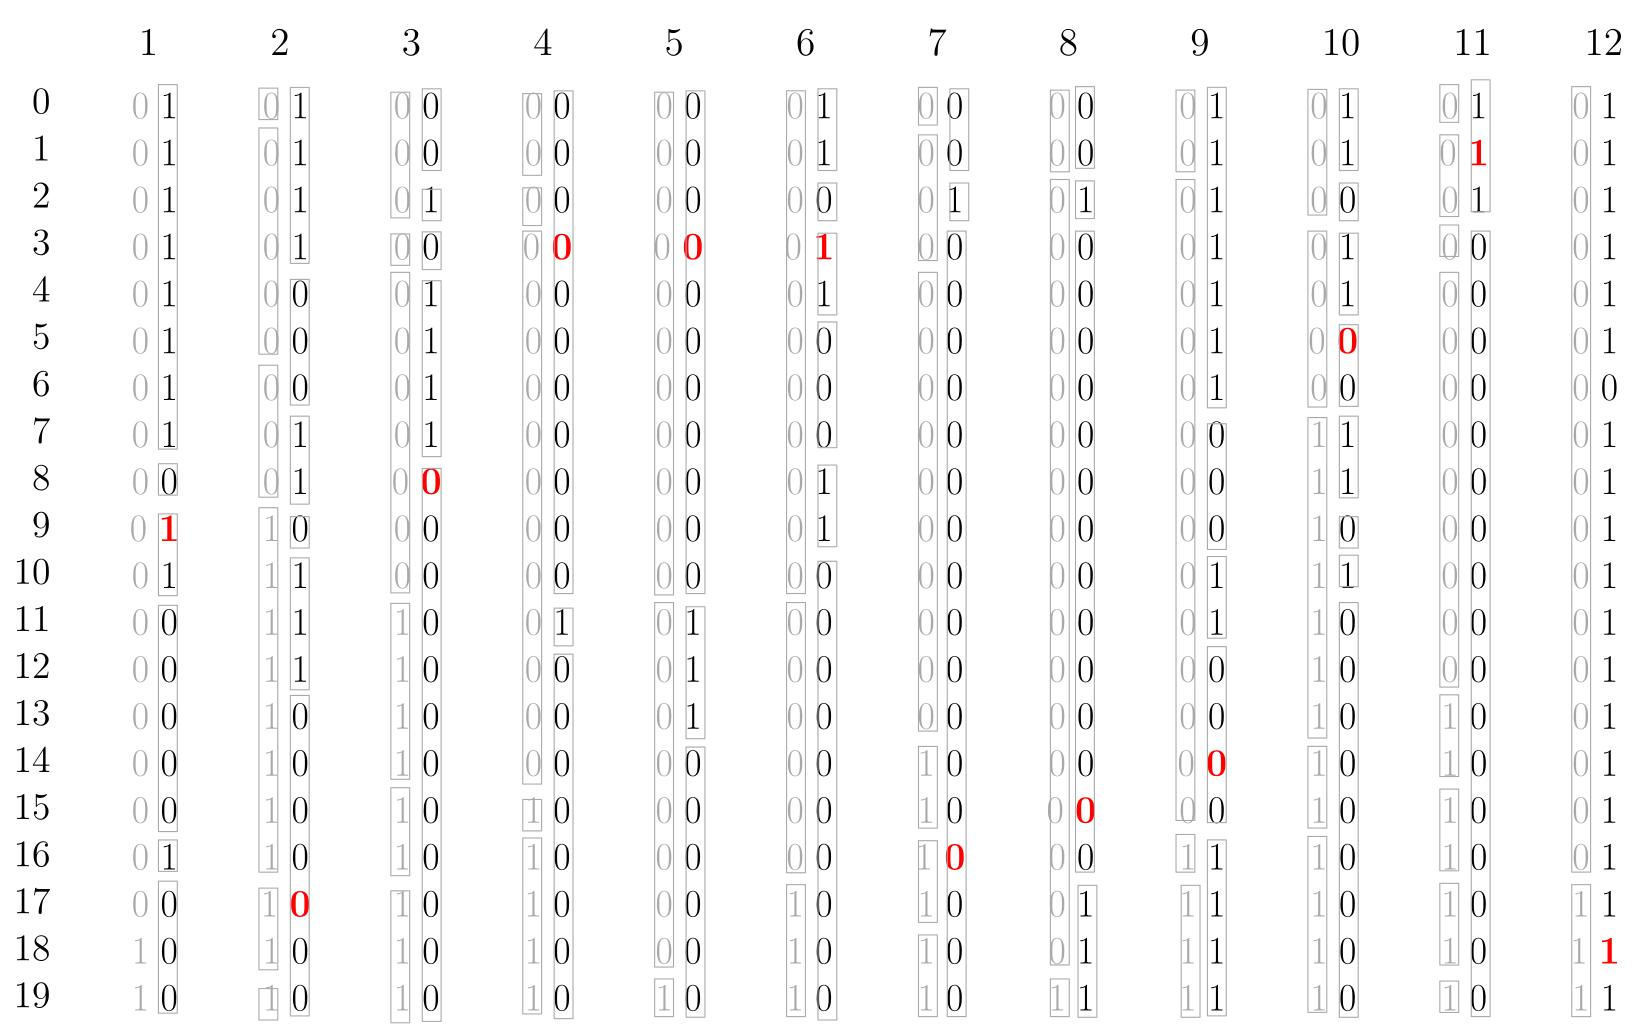
\includegraphics[scale = 0.2]{img/trick.jpg}
%   \end{figure}
% \end{frame}
% \begin{frame}{The compressed data structure}
%   \begin{block}{The tables}
%     \begin{itemize}
%       \item a set of $m$ tables in which the $m$-th table stores only the
%       positions of the run-heads in the $m$-th column and a bool to check the
%       first symbol: 0 or 1
%       \item the $i$-th row of the $j$-th table stores a quadruple
%     \end{itemize}    
%   \end{block}
%   \pause
%   \begin{block}{The quadruple}
%     \begin{enumerate}
%       \item the position $p$ of the $i$-th run-head in the $j$-th column of the
%       PBWT 
%       \item the permutation $\pi_j(p)$
%       \item the index of the run containing bit $\pi_j(p)$ in the $(j + 1)$-st
%       column of the PBWT
%       \item the threshold, that's the index of the minimum \textit{LCP value}
%       (current column minus divergence array value) in the run
%     \end{enumerate}
%   \end{block}
% \end{frame}
% \begin{frame}{Row extraction}
%   \begin{block}{First step}
%     We start by finding the row of the first table that starts with the position
%     $p$ of the head of the run containing bit $i$ in first column of the PBWT,
%     computing: 
%     \pause
%     \[\pi_1(i)=\pi_1(p)+i-p\]
%     \pause
%     looking up the row for the run containing bit $\pi_1(p)$ in the the second
%     table and scanning down the table until we find the row for the run
%     containing bit $\pi_1(i)$ 
%   \end{block}
%   \begin{block}{Next step}
%     We continue repeating this procedure for each column
%   \end{block}
% \end{frame}
% \begin{frame}{Travis's example I}
%   \begin{figure}[H]
%     \centering
%     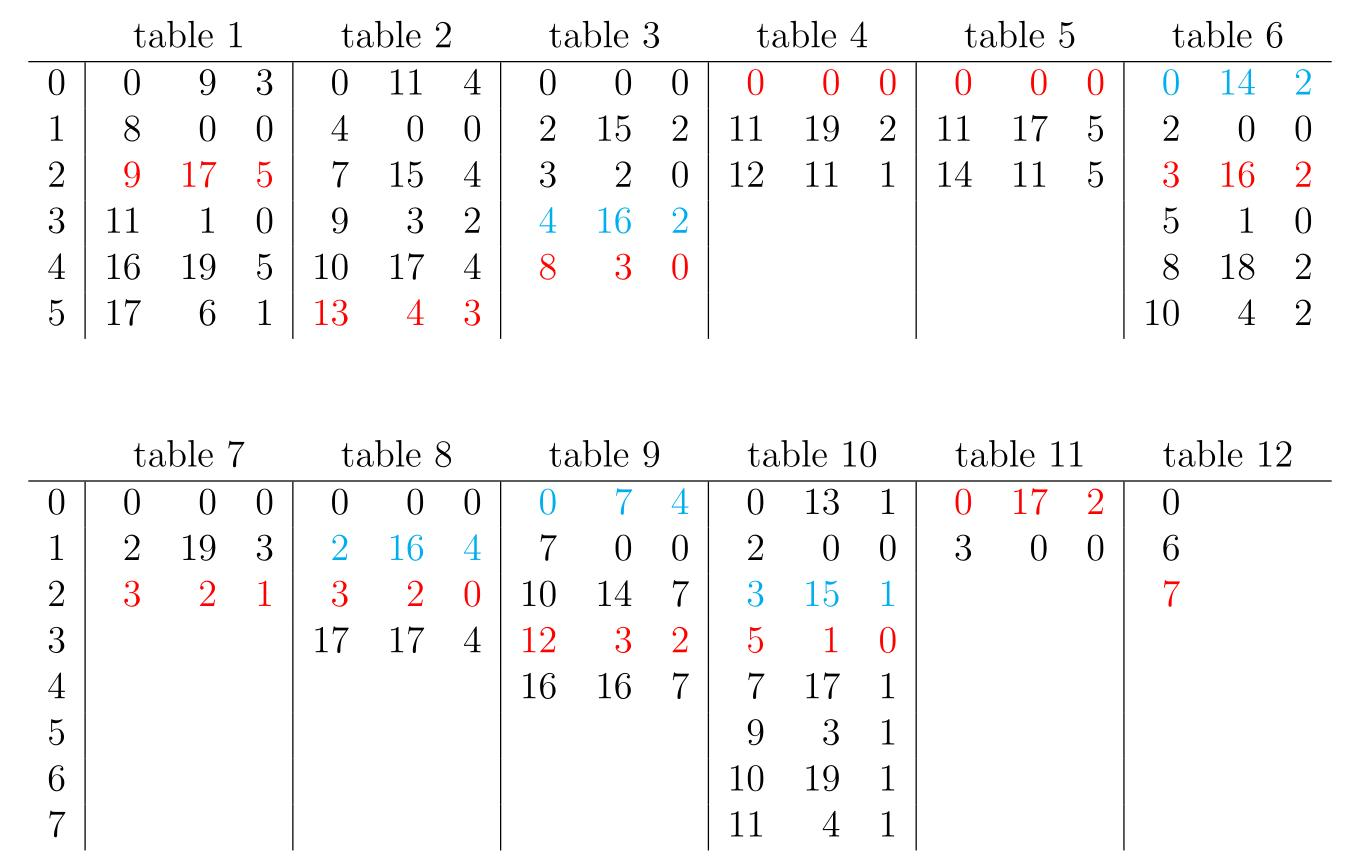
\includegraphics[scale = 0.22]{img/trick2.jpg}
%   \end{figure}
% \end{frame}
% \begin{frame}{Travis's example II}
%   \begin{block}{Extraction of row 9, $\pi_j(i)=\pi_j(p)+i-p$}
%     \begin{multicols}{2}
%       \begin{itemize}
%         \item $\pi_1(9)=17+9-9=17$
%         \item $\pi_2(17)=4+17-13=8$
%         \item $\pi_3(8)=4+8-8=3$
%         \item $\pi_4(3)=0+3-0=3$
%         \item $\pi_5(3)=0+3-0=3$
%         \item $\pi_6(3)=16+3-3=16$

%         \item $\pi_7(16)=2+16-3=15$
%         \item $\pi_8(15)=2+15-3=14$
%         \item $\pi_9(14)=3+14-12=5$
%         \item $\pi_{10}(5)=1+5-5=1$
%         \item $\pi_{11}(1)=17+1-0=18$
%         %         \item $\pi_{12}(3)=16+3-3=16$        
%       \end{itemize}
%     \end{multicols}
%   \end{block}
% \end{frame}
% \section{Example}
% \begin{frame}{The matrixes}
%   \begin{block}{Panel and query}
%     \begin{table}[H]
%       \centering
%       \tiny
%       \begin{tabular}{c|c|c|c|c|c|c|c|c|c|c|c|c|c|c|c|c|c|c|c}
          %           \hline
          %           0 & 1 & 2 & 3 & 4 & 5 & 6 & 7 & 8 & 9 & 10 & 11 & 12 & 13 & 14 & 15 & 16
                                                                                            %           & 17 & 18 & 19\\
          %           \hline
          %           \hline

          %           1 & 1 & 0 & 1 & 0 & 0 & 1 & 1 & 1 & 1 & 1 & 0 & 0 & 1 & 0 & 0 & 1 & 0
                                                                                          %                                                                                                              & 0 & 1\\
          %           0 & 1 & 0 & 0 & 0 & 0 & 1 & 1 & 1 & 1 & 1 & 0 & 0 & 1 & 1 & 1 & 0 & 0
                                                                                          %                                                                                                              & 1 & 0\\
          %           0 & 0 & 0 & 1 & 0 & 0 & 0 & 0 & 0 & 1 & 1 & 1 & 1 & 0 & 0 & 0 & 1 & 0
                                                                                          %                                                                                                              & 1 & 0\\
          %           1 & 0 & 0 & 1 & 1 & 0 & 1 & 0 & 1 & 0 & 0 & 0 & 1 & 1 & 1 & 0 & 0 & 0
                                                                                          %                                                                                                              & 1 & 0\\
          %           0 & 1 & 1 & 0 & 1 & 1 & 1 & 1 & 1 & 0 & 0 & 1 & 0 & 0 & 1 & 1 & 1 & 1
                                                                                          %                                                                                                              & 0 & 0\\
          %           1 & 1 & 0 & 0 & 1 & 0 & 1 & 0 & 1 & 0 & 1 & 0 & 1 & 0 & 0 & 0 & 1 & 1
                                                                                          %                                                                                                              & 1 & 1\\
          %           0 & 0 & 0 & 1 & 0 & 1 & 1 & 1 & 1 & 1 & 1 & 1 & 0 & 0 & 1 & 0 & 0 & 0
                                                                                          %                                                                                                              & 1 & 1\\
          %           \hline
          %           \hline
          %           \hline
          %           0 & 0 & 1 & 0 & 1 & 1 & 1 & 1 & 1 & 1 & 1 & 0 & 0 & 1 & 0 & 0 & 0 & 1
                                                                                          %                                                                                                              & 1 & 1
                                                                                                                                                                                                               %         \end{tabular}
                                                                                                                                                                                                               %                                                                                                                                                                                                                \end{table}
                                                                                                                                                                                                               %                                                                                                                                                                                                                \end{block}
                                                                                                                                                                                                               %                                                                                                                                                                                                                \begin{block}{PBWT Matrix}
                                                                                                                                                                                                               %                                                                                                                                                                                                                \begin{table}[H]
                                                                                                                                                                                                               %                                                                                                                                                                                                                \centering
                                                                                                                                                                                                               %                                                                                                                                                                                                                \tiny
                                                                                                                                                                                                               %                                                                                                                                                                                                                \begin{tabular}{c|c|c|c|c|c|c|c|c|c|c|c|c|c|c|c|c|c|c|c}
                                                                                                                                                                                                               %                                                                                                                                                                                                                \hline
                                                                                                                                                                                                               %                                                                                                                                                                                                                0 & 1 & 2 & 3 & 4 & 5 & 6 & 7 & 8 & 9 & 10 & 11 & 12 & 13 & 14 & 15 & 16
                                                                                                                                                                                                                                                                                                                                                                                                                                                                                                      %                                                                                         & 17 & 18 & 19\\
          %           \hline
          %           \hline
          %           1 & 1 & 0 & 1 & 0 & 0 & 1 & 0 & 0 & 1 & 1 & 0 & 1 & 1 & 1 & 0 & 1 & 0
                                                                                          %                                                                                                              & 1 & 1 \\
          %           0 & 0 & 0 & 1 & 1 & 0 & 0 & 1 & 1 & 0 & 0 & 1 & 1 & 1 & 1 & 0 & 1 & 0
                                                                                          %                                                                                                              & 1 & 0 \\
          %           0 & 1 & 0 & 1 & 1 & 1 & 1 & 1 & 1 & 0 & 0 & 0 & 0 & 0 & 0 & 0 & 1 & 0
                                                                                          %                                                                                                              & 1 & 1 \\
          %           1 & 0 & 0 & 0 & 0 & 0 & 1 & 0 & 1 & 1 & 1 & 1 & 0 & 0 & 0 & 1 & 0 & 1
                                                                                          %                                                                                                              & 1 & 0 \\
          %           0 & 1 & 1 & 1 & 0 & 0 & 1 & 0 & 1 & 1 & 1 & 0 & 0 & 1 & 1 & 0 & 0 & 0
                                                                                          %                                                                                                              & 0 & 0 \\
          %           1 & 0 & 0 & 0 & 1 & 1 & 1 & 1 & 1 & 1 & 1 & 0 & 1 & 0 & 0 & 1 & 1 & 0
                                                                                          %                                                                                                              & 1 & 0 \\
          %           0 & 1 & 0 & 0 & 0 & 0 & 1 & 1 & 1 & 0 & 1 & 1 & 0 & 0 & 1 & 0 & 0 & 1
                                                                                          %                                                                                                              & 0 & 1 \\
          %           \hline
          %         \end{tabular}
          %           \end{table}
          %           \end{block}
          %           \end{frame}
          %           \begin{frame}{Prefix and Divergence Arrays}
          %           \begin{block}{Prefix Arrays}
          %           \begin{table}[H]
          %           \tiny
          %           \begin{tabular}{c|c|c|c|c|c|c|c|c|c|c|c|c|c|c|c|c|c|c|c}
          %           \hline
          %           0 & 1 & 2 & 3 & 4 & 5 & 6 & 7 & 8 & 9 & 10 & 11 & 12 & 13 & 14 & 15 & 16
                                                                                            %                                                                                                         & 17 & 18 & 19\\
          %           \hline
          %           \hline
          %           0 & 1 & 2 & 2 & 1 & 1 & 1 & 2 & 2 & 2 & 5 & 3 & 3 & 1 & 4 & 5 & 5 & 6
                                                                                          %                                                                                                              & 6 & 0\\  
          %           1 & 2 & 6 & 6 & 5 & 2 & 2 & 1 & 5 & 5 & 3 & 4 & 5 & 0 & 6 & 2 & 2 & 3
                                                                                          %                                                                                                              & 3 & 4\\  
          %           2 & 4 & 3 & 3 & 4 & 6 & 0 & 0 & 3 & 3 & 4 & 5 & 1 & 4 & 5 & 0 & 0 & 1
                                                                                          %                                                                                                              & 1 & 6\\  
          %           3 & 6 & 1 & 1 & 2 & 0 & 5 & 5 & 1 & 1 & 2 & 2 & 0 & 6 & 2 & 4 & 6 & 5
                                                                                          %                                                                                                              & 2 & 3\\  
          %           4 & 0 & 4 & 0 & 6 & 5 & 3 & 3 & 0 & 0 & 1 & 1 & 4 & 3 & 1 & 6 & 3 & 2
                                                                                          %                                                                                                              & 0 & 1\\  
          %           5 & 3 & 0 & 5 & 3 & 4 & 6 & 6 & 6 & 6 & 0 & 0 & 2 & 5 & 0 & 1 & 4 & 0
                                                                                          %                                                                                                              & 5 & 2\\
          %           6 & 5 & 5 & 4 & 0 & 3 & 4 & 4 & 4 & 4 & 6 & 6 & 6 & 2 & 3 & 3 & 1 & 4
                                                                                          %                                                                                                              & 4 & 5\\
          %           \hline
          %         \end{tabular}
          %           \end{table}
          %           \end{block}
          %           \begin{block}{LCP Arrays: current \textit{k} minus the original Durbin's
          %           divergence arrays}  
          %           \begin{table}[H]
          %           \tiny
          %           \begin{tabular}{c|c|c|c|c|c|c|c|c|c|c|c|c|c|c|c|c|c|c|c}
          %           \hline
          %           0 & 1 & 2 & 3 & 4 & 5 & 6 & 7 & 8 & 9 & 10 & 11 & 12 & 13 & 14 & 15 & 16
                                                                                            %                                                                                                         & 17 & 18 & 19\\
          %           \hline
          %           \hline
          %           0 & 0 & 0 & 0 & 0 & 0 & 0 & 0 & 0 & 0 & 0 & 0 & 0 & 0 & 0 & 0 & 0 & 0
                                                                                          %                                                                                                              & 0 & 0 \\
          %           0 & 1 & 2 & 3 & 3 & 1 & 2 & 0 & 1 & 0 & 6 & 3 & 1 & 9 & 3 & 3 & 4 & 3
                                                                                          %                                                                                                              & 4 & 1 \\
          %           0 & 1 & 1 & 2 & 1 & 5 & 4 & 3 & 4 & 5 & 2 & 0 & 2 & 1 & 1 & 1 & 2 & 1
                                                                                          %                                                                                                              & 2 & 0 \\
          %           0 & 1 & 0 & 1 & 0 & 3 & 1 & 2 & 0 & 1 & 0 & 1 & 8 & 2 & 2 & 0 & 1 & 0
                                                                                          %                                                                                                              & 1 & 5 \\
          %           0 & 0 & 2 & 2 & 4 & 0 & 2 & 3 & 4 & 5 & 1 & 2 & 0 & 0 & 0 & 4 & 2 & 5
                                                                                          %                                                                                                              & 4 & 3 \\
          %           0 & 1 & 1 & 3 & 3 & 2 & 0 & 1 & 2 & 3 & 6 & 7 & 1 & 2 & 10 & 1 & 0 & 3
                                                                                           %                                                                                                              & 0 & 2 \\
          %           0 & 1 & 2 & 0 & 2 & 1 & 1 & 2 & 3 & 4 & 4 & 5 & 3 & 1 & 1 & 2 & 2 & 1
                                                                                          %                                                                                                              & 2 & 1\\
          %         \end{tabular}
          %           \end{table}
          %           \end{block}
          %           \end{frame}

          %           \begin{frame}{Run-Length PBWT I, \textit{p, perm, next perm, threshold}}
          %           \begin{block}{ $[0,1,2,3,4]$} 
          %           {\footnotesize{\[
          %           \begin{matrix}
          %           0 & 4 & 4 & 0\\
          %           1 & 0 & 0 & 1\\
          %           3 & 5 & 5 & 3\\
          %           \color{nordgreen} 4 &\color{nordgreen} 2 &\color{nordgreen} 2
                                                                 %                                 &\color{nordgreen} 4\\ 
          %           5 & 6 & 6 & 5\\
          %           6 & 3 & 3 & 6
                                  %                                   \end{matrix}
                                  %                                   \Longrightarrow
                                  %                                   \begin{matrix}
                                  %                                   0 & 3 & 0 & 0\\
          %           1 & 0 & 0 & 1\\
          %           \color{nordgreen} 2 &  \color{nordgreen} 4 &  \color{nordgreen} 1 &
                                                                                          %                                                                                           \color{nordgreen} 2\\
          %           3 & 1 & 0 & 3\\
          %           4 & 5 & 2 & 4\\
          %           5 & 2 & 0 & 5\\
          %           6 & 6 & 2 & 6
                                  %                                   \end{matrix}
                                  %                                   \Longrightarrow
                                  %                                   \begin{matrix}
                                  %                                   0 & 0 & 0 & 0\\
          %           \color{nordgreen} 4 & \color{nordgreen} 6 & \color{nordgreen} 3 &
                                                                                        %                                                                                         \color{nordgreen} 4\\
          %           5 & 4 &  2 & 5
                                   %                                    \end{matrix}
                                   %                                    \Longrightarrow
                                   %                                    \begin{matrix}
                                   %                                    0 & 3 & 2 & 0\\
          %           3 & 0 & 0 & 3\\
          %           4 & 6 & 4 & 4\\
          %           \color{nordgreen} 5 & \color{nordgreen} 1 & \color{nordgreen} 1 &
                                                                                        %                                                                                         \color{nordgreen} 6
                                                                                        %                                                                                         \end{matrix}
                                                                                        %                                                                                         \Longrightarrow
                                                                                        %                                                                                         \begin{matrix}
                                                                                        %                                                                                         0 & 0 & 0 & 0\\
          %           \color{nordgreen} 1 &  \color{nordgreen} 4 &  \color{nordgreen} 2 &
                                                                                          %                                                                                           \color{nordgreen} 2\\
          %           3 & 1 & 0 & 3\\
          %           5 & 6 & 4 & 5\\
          %           6 & 3 & 2 & 6
                                  %                                   \end{matrix}\]}}
                                  %                                   \end{block}
                                  %                                   \begin{block}{$[5,6,7,8,9]$}
                                  %                                   {\footnotesize{\[
                                  %                                   \begin{matrix}
                                  %                                   0 & 0 & 0 & 0\\
          %           2 & 5 & 2 & 2\\
          %           \color{nordred} 3 & \color{nordred} 2 & \color{nordred} 2 &
                                                                                  %                                                                                   \color{nordred} 4\\
          %           \color{nordgreen} 5 &  \color{nordgreen} 6 &   \color{nordgreen}2 &
                                                                                          %                                                                                           \color{nordgreen} 5\\
          %           6 & 4 & 2 & 6
                                  %                                   \end{matrix}
                                  %                                   \Longrightarrow
                                  %                                   \begin{matrix}
                                  %                                   0 & 1 & 1 & 0\\
          %           1 & 0 & 0 & 1\\
          %           \color{nordgreen} 2 & \color{nordgreen} 2 & \color{nordgreen} 1 &
                                                                                        %                                                                                         \color{nordgreen} 5
                                                                                        %                                                                                         \end{matrix}
                                                                                        %                                                                                         \Longrightarrow
                                                                                        %                                                                                         \begin{matrix}
                                                                                        %                                                                                         0 & 0 & 0 & 0\\
          %           \color{nordred} 1 &  \color{nordred} 3 &  \color{nordred} 1 &
                                                                                    %                                                                                     \color{nordred} 1\\ 
          %           3 & 1 & 1 & 3\\
          %           \color{nordgreen} 5 & \color{nordgreen} 5 & \color{nordgreen} 1 &
                                                                                        %                                                                                         \color{nordgreen} 5
                                                                                        %                                                                                         \end{matrix}
                                                                                        %                                                                                         \Longrightarrow
                                                                                        %                                                                                         \begin{matrix}
                                                                                        %                                                                                         0 & 0 & 0 & 0\\
          %           \color{nordgreen} 1 & \color{nordgreen} 1 & \color{nordgreen} 1 &
                                                                                        %                                                                                         \color{nordgreen} 3
                                                                                        %                                                                                         \end{matrix}
                                                                                        %                                                                                         \Longrightarrow
                                                                                        %                                                                                         \begin{matrix}
                                                                                        %                                                                                         0 & 3 & 2 & 0\\
          %           \color{nordred} 1 &  \color{nordred} 0 &  \color{nordred} 0 &
                                                                                    %                                                                                     \color{nordred} 1\\ 
          %           3 & 4 & 2 & 3\\
          %           \color{nordgreen} 6 & \color{nordgreen} 2 & \color{nordgreen} 1 &
                                                                                        %                                                                                         \color{nordgreen} 6           
                                                                                        %                                                                                         \end{matrix}\]}}
                                                                                        %                                                                                         \end{block}
                                                                                        %                                                                                         \end{frame}
                                                                                        %                                                                                         \begin{frame}{Run-Length PBWT II}
                                                                                        %                                                                                         \begin{block}{$[10,11,12,13,14]$}
                                                                                        %                                                                                         {\footnotesize{\[
                                                                                        %                                                                                         \begin{matrix}
                                                                                        %                                                                                         0 & 2 & 2 & 0\\
          %           \color{nordgreen} 1 & \color{nordgreen} 0 & \color{nordgreen} 0 &
                                                                                        %                                                                                         \color{nordgreen} 2\\
          %           3 & 3 & 3 & 3
                                  %                                   \end{matrix}
                                  %                                   \Longrightarrow
                                  %                                   \begin{matrix}
                                  %                                   \color{nordred} 0 & \color{nordred} 0 & \color{nordred} 0 &
                                                                                                                                  %                                                                                                                                   \color{nordred} 0\\
          %           \color{nordgreen} 1 & \color{nordgreen} 4 & \color{nordgreen} 1 &
                                                                                        %                                                                                         \color{nordgreen} 1\\
          %           2 & 1 & 0 & 2\\
          %           3 & 5 & 2 & 3\\
          %           4 & 2 & 1 & 4\\
          %           6 & 6 & 3 & 6
                                  %                                   \end{matrix}
                                  %                                   \Longrightarrow
                                  %                                   \begin{matrix}
                                  %                                   0 & 4 & 2 & 0\\
          %           \color{nordgreen} 2 & \color{nordgreen} 0 & \color{nordgreen} 0 &
                                                                                        %                                                                                         \color{nordgreen} 4\\
          %           5 & 6 & 3 & 5\\
          %           6 & 3 & 1 & 6
                                  %                                   \end{matrix}
                                  %                                   \Longrightarrow
                                  %                                   \begin{matrix}
                                  %                                   \color{nordred} 0 & \color{nordred} 4 & \color{nordred} 2 &
                                                                                                                                  %                                                                                                                                   \color{nordred} 0\\
          %           \color{nordgreen} 2 & \color{nordgreen} 0 & \color{nordgreen} 0 &
                                                                                        %                                                                                         \color{nordgreen}2\\ 
          %           4 & 6 & 4 & 4\\
          %           5 & 2 & 1 & 6
                                  %                                   \end{matrix}
                                  %                                   \Longrightarrow
                                  %                                   \begin{matrix}
                                  %                                   \color{nordgreen} 0 & \color{nordgreen} 3 & \color{nordgreen} 1 &
                                                                                                                                        %                                                                                                                                         \color{nordgreen} 0\\ 
          %           2 & 0 & 0 & 2\\
          %           4 & 5 & 3 & 4\\
          %           5 & 2 & 0 & 5\\
          %           6 & 6 & 4 & 6
                                  %                                   \end{matrix}\]}}
                                  %                                   \end{block}
                                  %                                   \begin{block}{$[15,16,17,18,19]$}
                                  %                                   {\footnotesize{\[
                                  %                                   \begin{matrix}
                                  %                                   0 & 0 & 0 & 0\\
          %           \color{nordgreen} 3 & \color{nordgreen} 5 & \color{nordgreen} 2 &
                                                                                        %                                                                                         \color{nordgreen} 3\\
          %           4 & 3 & 1 & 4\\
          %           5 & 6 & 3 & 5\\
          %           6 & 4 & 1 & 6
                                  %                                   \end{matrix}
                                  %                                   \Longrightarrow
                                  %                                   \begin{matrix}
                                  %                                   0 & 3 & 1 & 0\\
          %           3 & 0 & 0 & 3\\
          %           \color{nordgreen}5 & \color{nordgreen} 6 & \color{nordgreen} 3 &
                                                                                       %                                                                                        \color{nordgreen} 5\\ 
          %           6 & 2 & 0 & 6
                                  %                                   \end{matrix}
                                  %                                   \Longrightarrow
                                  %                                   \begin{matrix}
                                  %                                   0 & 0 & 0 & 0\\
          %           3 & 5 & 2 & 3\\
          %           4 & 3 & 0 & 5\\
          %           \color{nordgreen} 6 & \color{nordgreen} 6 & \color{nordgreen} 3 &
                                                                                        %                                                                                         \color{nordgreen} 6
                                                                                        %                                                                                         \end{matrix}
                                                                                        %                                                                                         \Longrightarrow
                                                                                        %                                                                                         \begin{matrix}  
                                                                                        %                                                                                         0 & 2 & 2 & 0\\
          %           4 & 0 & 0 & 4\\
          %           5 & 6 & 4 & 5\\
          %           \color{nordgreen} 6 & \color{nordgreen} 1 & \color{nordgreen} 1 &
                                                                                        %                                                                                         \color{nordgreen} 6
                                                                                        %                                                                                         \end{matrix}
                                                                                        %                                                                                         \Longrightarrow
                                                                                        %                                                                                         \begin{matrix}  
                                                                                        %                                                                                         0 & 4 & 0 & 0\\
          %           \color{nordgreen} 1 & \color{nordgreen} 0 & \color{nordgreen} 0 &
                                                                                        %                                                                                         \color{nordgreen} 1\\
          %           2 & 5 & 0 & 2\\
          %           3 & 1 & 0 & 5\\
          %           6 & 6 & 0 & 6
                                  %                                   \end{matrix}\]}}
                                  %                                   \end{block}
                                  %                                   \end{frame}
                                  %                                   \begin{frame}{Match with external haplotype I}
                                  %                                   \begin{block}{First case, bits matches at column $j$-th}
                                  %                                   \begin{itemize}
                                  %                                   \item we are looking at $d$-th bit of the $k$-th run, that come from the
                                  %                                   $i$-th row of the panel 
                                  %                                   \item if this bit match the next bit of the pattern we can go to column
                                  %                                   $j+1$ and we figure out which bit to look at in that column 
                                  %                                   \item the next bit we look at is still from row $i$-th
                                  %                                   \end{itemize}
                                  %                                   \end{block}
                                  %                                   \end{frame}
                                  %                                   \begin{frame}{Match with external haplotype II}
                                  %                                   \begin{block}{Second case, bits doesn't matches at column $j$-th}
                                  %                                   \begin{itemize}
                                  %                                   \item we are looking at $d$-th bit of the $k$-th run and that bit
                                  %                                   doesn't match the next bit in the pattern 
                                  %                                   \item we look at the threshold for the $k$-th run:
                                  %                                   \begin{itemize}
                                  %                                   \item if $d$ is at most the threshold (check this "at most") than we
                                  %                                   move to the last bit of the ($k-1$)-st run in the $j$-th column and
                                  %                                   then we proceed as in \textit{case 1}  
                                  %                                   \item if $d$ is greater than the threshold than we move to the first
                                  %                                   bit of the ($k-1$)-st run in the $j$-th column and then we proceed
                                  %                                   as in \textit{case 1}  
                                  %                                   \end{itemize}
                                  %                                   \end{itemize}
                                  %                                   \end{block}
                                  %                                   \end{frame}
                                  %                                   \begin{frame}{Travis's New Version}
                                  %                                   \begin{block}{}
                                  %                                   A column C's representation consists of a bitvector $B[0..m - 1]$ and a
                                  %                                   sequence of thresholds $T$.  It supports the query \textit{CANDIDATE\_STEP},
                                  %                                   which takes a single 
                                  %                                   integer $i$ and a bit $b$ and returns a boolean flag $f$ and a single
                                  %                                   integer $i'$. 
                                  %                                   If $B[i] = b$, then $f = TRUE$ and $i'$ is the position of $B[i]$ after $B$
                                  %                                   is stably 
                                  %                                   sorted. If $B[i] \neq b$ but there is some copy of $b$ in $B$, the $f =
                                  %                                   FALSE$ and $i'$ 
                                  %                                   is the position after $B$ is stably sorted of either of the last copy of $b$
                                  %                                   before B[i] or of the first copy of b after $B[i]$, depending on whether
                                  %                                   $B[i]$ is 
                                  %                                   before or after the threshold for the run containing $B[i]$.  If there is no
                                  %                                   copy of $b$ in $B$, then $f = FALSE$ and $i' = -1$. 

                                  %                                   We store $B$ and $T$ run-length compressed, so they take $O(r_c)$ words of
                                  %                                   space and \textit{CANDIDATE\_STEP} takes $O(\log \log m)$ time.  We start a
                                  %                                   search with $i = 0$; we go 
                                  %                                   from one column to the next setting $i = i'$ when $i' \geq 0$, with $f$
                                  %                                   telling us whether we've jumped or not (\textbf{but not telling us whether
                                  %                                   we've hit the end of a MEM}); when $i' = -1$, we were unable to match a
                                  %                                   column and we start over at the next column with $i = 0$.  
                                  %                                   \end{block}
                                  %                                   \end{frame}
\section{The Old Idea}
\begin{frame}{Durbin's Algorithm}
  \begin{algorithm}[H]
    \scriptsize
    \begin{algorithmic}
      \Function{Find\_Set\_Maximal\_Matches\_From\_Z}{$z$}
      \For {$k\gets 0$ \textbf{to} $N$}
      \State $e,f,g\gets \mbox{\textit{Update\_Z\_Matches}}(k, z, e, f, g)$
      \EndFor
      \EndFunction
      \Function{Update\_Z\_Matches}{$k, z, e, f, g$}
      \State $f'\gets w(k, f, z[k])$
      \Comment{$a_k$, $d_k$ and $y_i^k$ as in Durbin's paper}
      \State $g'\gets w(k, g, z[k])$
      \If{$f'<g'$}
      \Comment\textit{{if $k$ is $N-1$ report matches from $e_k$ to $N-1$}}
      \State $e'\gets e_k$
      \Else
      \Comment{\textit{report matches  from $e_k$ to $k$}}
      \State $e'\gets d_{k+1}[f']-1$
      \If{$z[e']=0$ \textbf{and} $f'>0$}
      \State $f'\gets g'-1$
      \State \textbf{while} $z[e'-1]=y_{f'}^{k+1}[e'-1]$ \textbf{do} $e'\gets
      e'-1$
      \State \textbf{while} $d_{k+1}[f']\leq e'$ \textbf{do} $f'\gets f'-1$
      \Else
      \State $g'\gets f'+1$
      \State \textbf{while} $z[e'-1]=y_{f'}^{k+1}[e'-1]$ \textbf{do}  $e'\gets
      e'-1$ 
      \State \textbf{while} $g'<M$ \textbf{and} $d_{k+1}[g']\leq e'$ \textbf{do}
      $g'\gets g'+1$ 
      \EndIf
      \EndIf
      \State \textbf{return} $e',f',g'$
      \EndFunction
    \end{algorithmic}
    \caption{Algorithm 5 from Durbin's paper}
  \end{algorithm}
\end{frame}
\begin{frame}{Durbin's Algorithm Example}
  \only<1>{
    \begin{figure}[H]
      \centering
      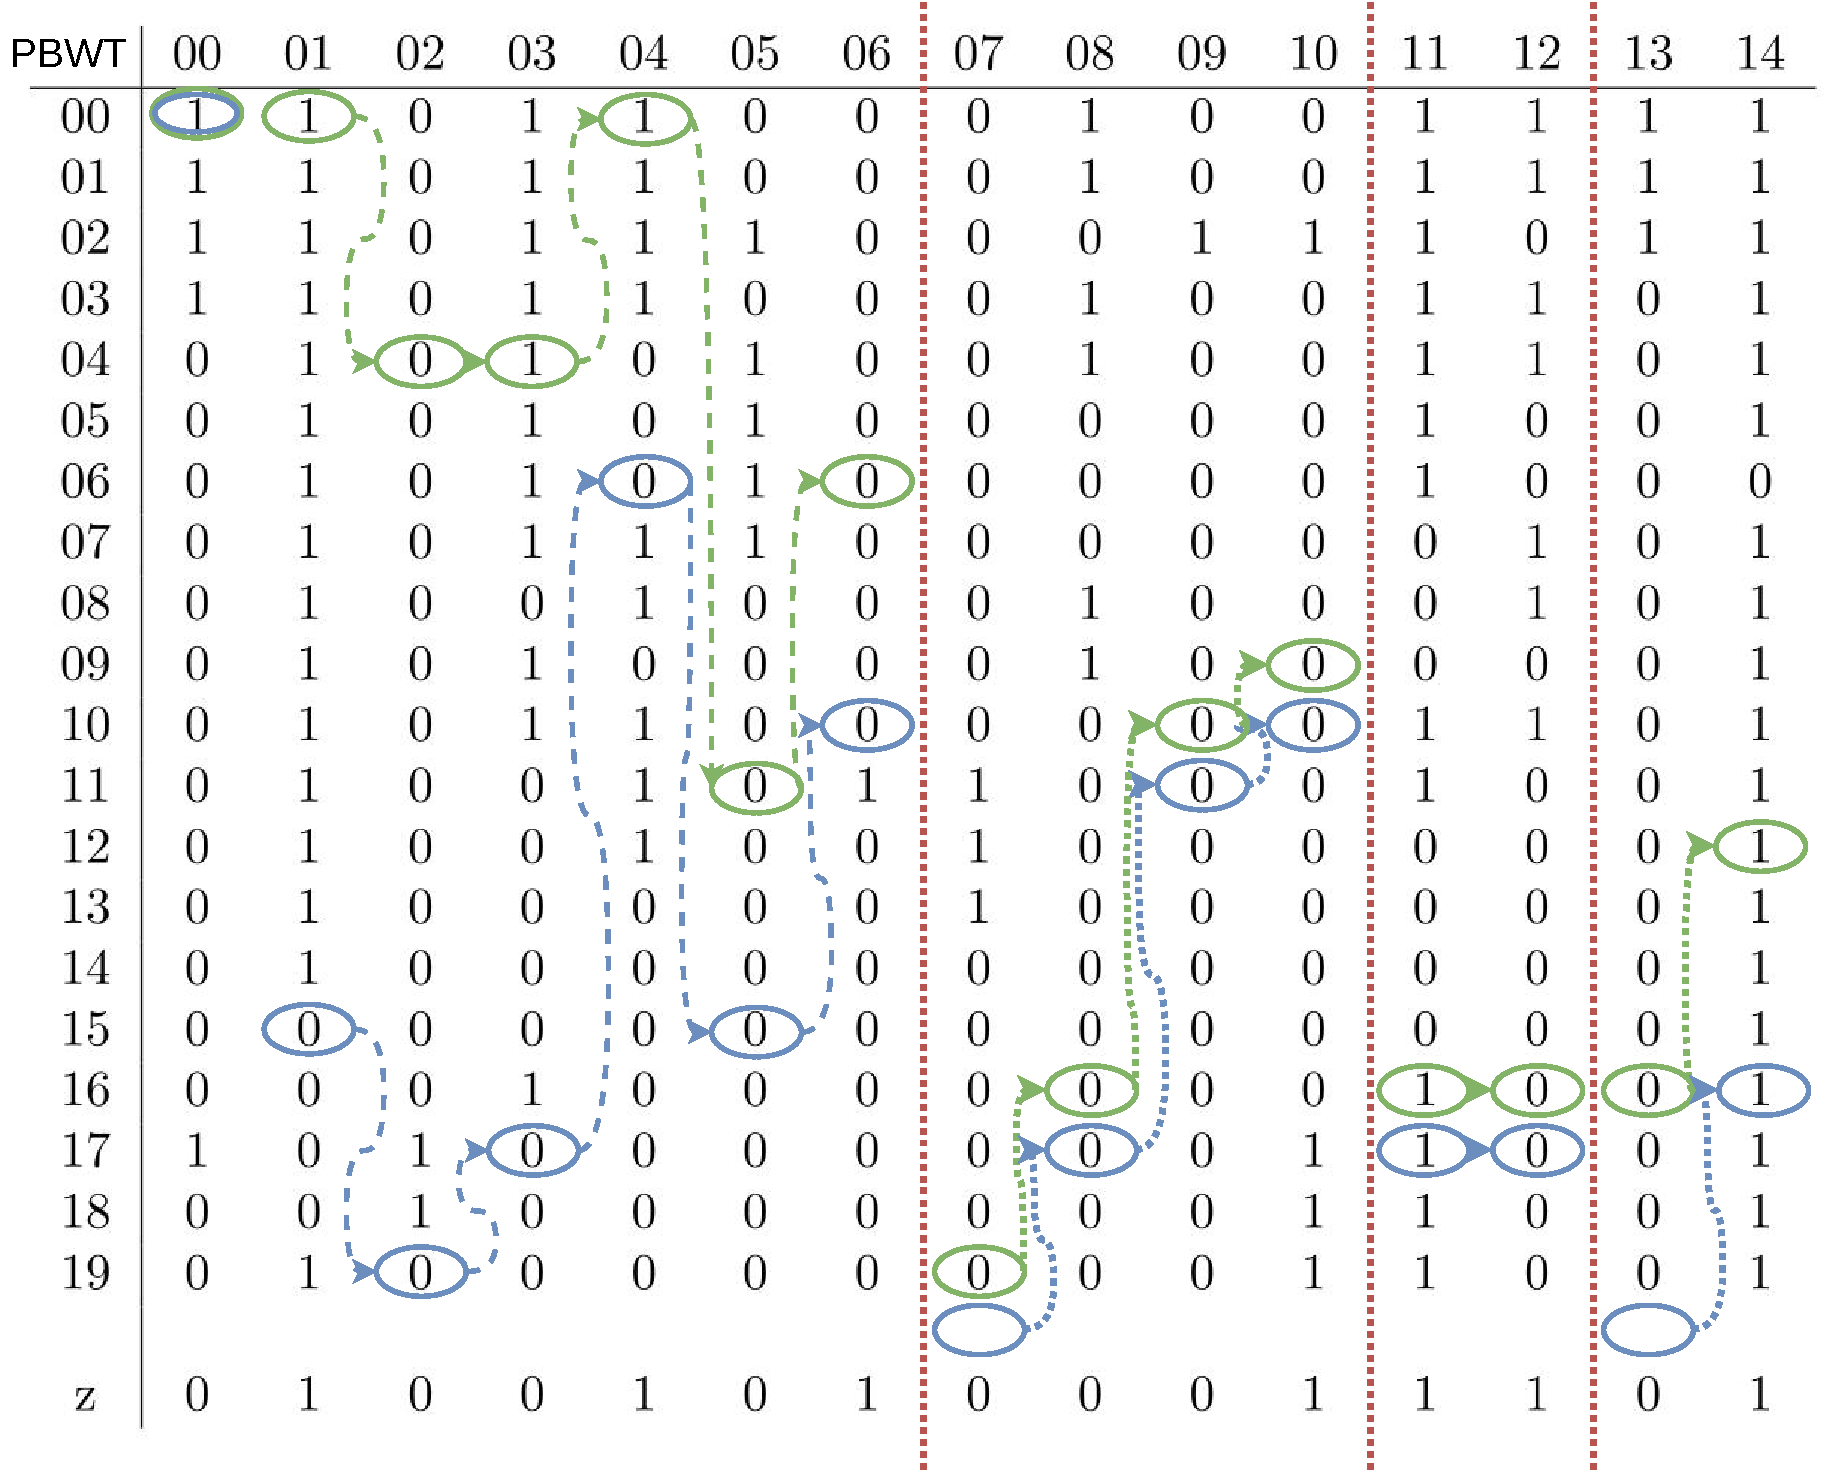
\includegraphics[scale = 0.3]{graph/fgtravis2.pdf}
    \end{figure}
  }
  \only<2>{
    \begin{figure}[H]
      \centering
      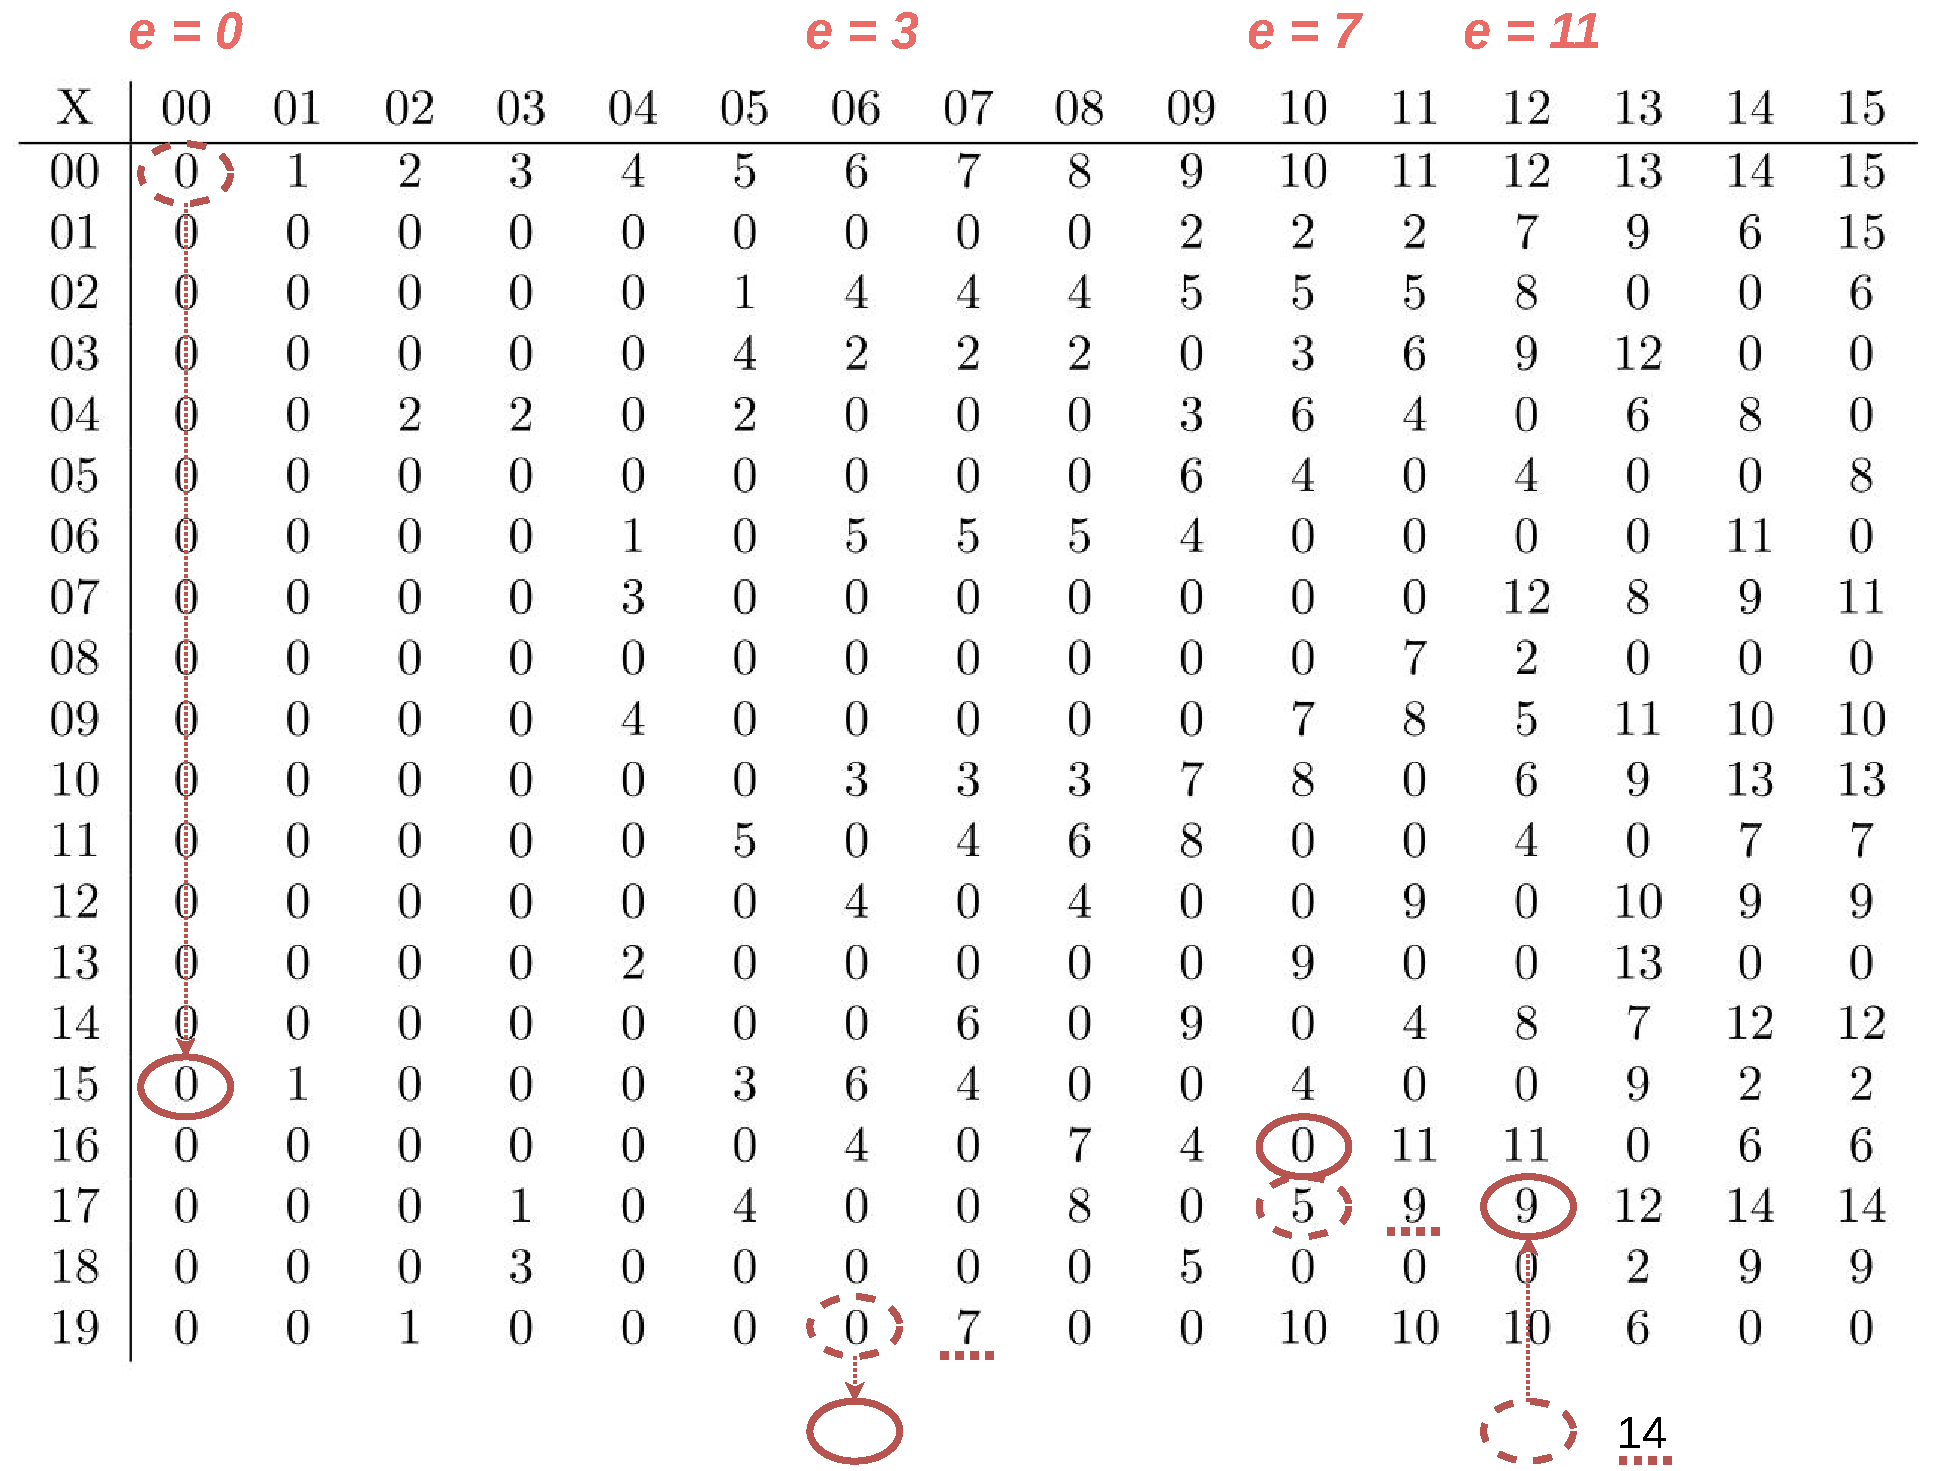
\includegraphics[scale = 0.3]{graph/divtravis.pdf}
    \end{figure}
  }\only<3>{
    \begin{figure}[H]
      \centering
      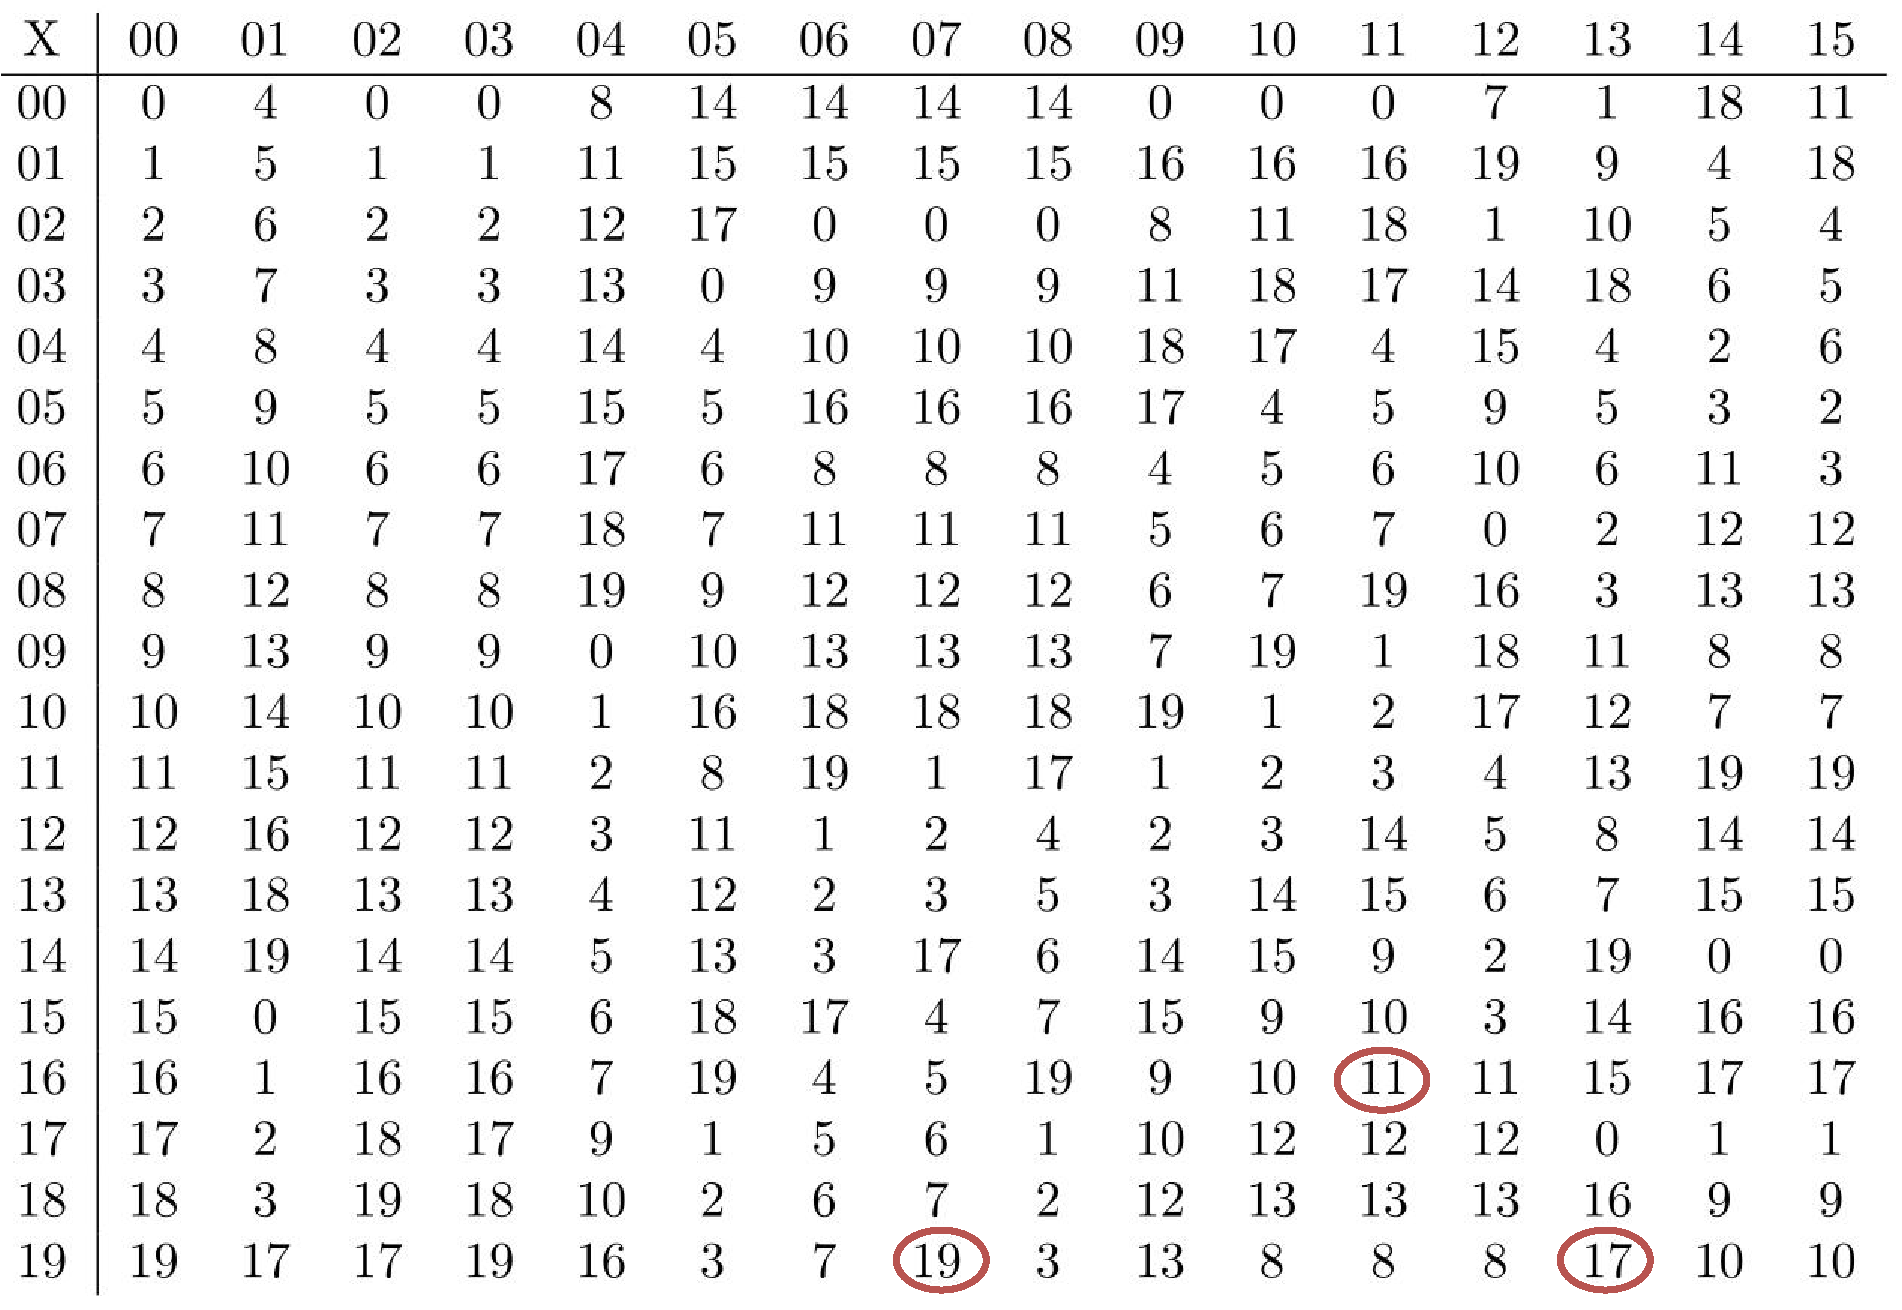
\includegraphics[scale = 0.3]{graph/preftravis.pdf}
    \end{figure}
  }\only<4>{
    \begin{figure}[H]
      \centering
      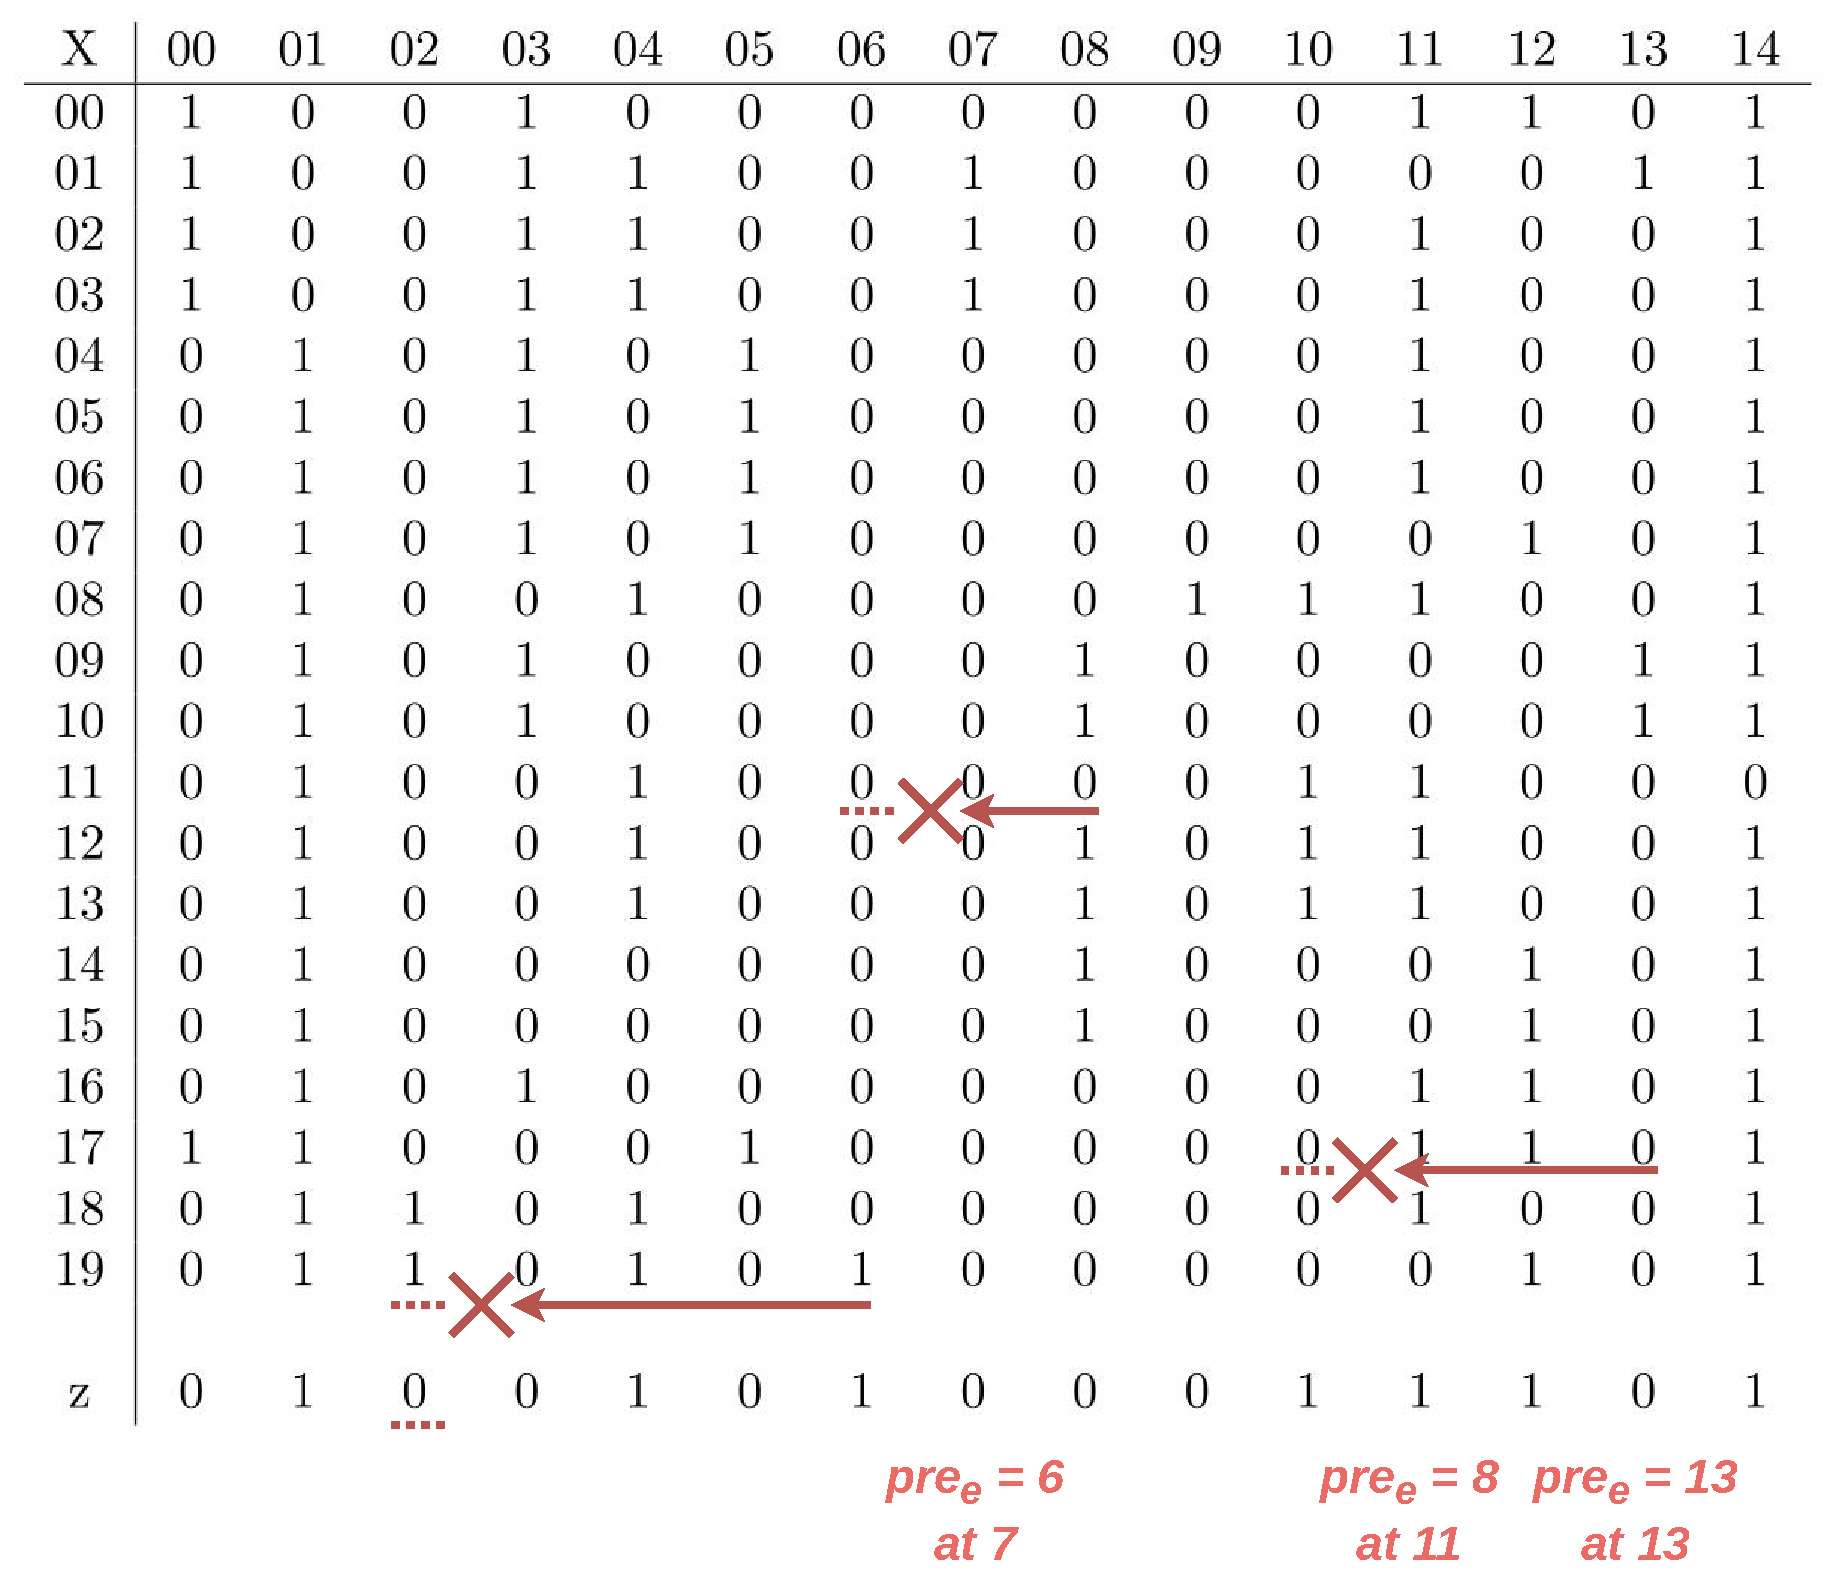
\includegraphics[scale = 0.3]{graph/backtravis.pdf}
    \end{figure}
  }
\end{frame}
\begin{frame}
  \begin{figure}[H]
    \centering
    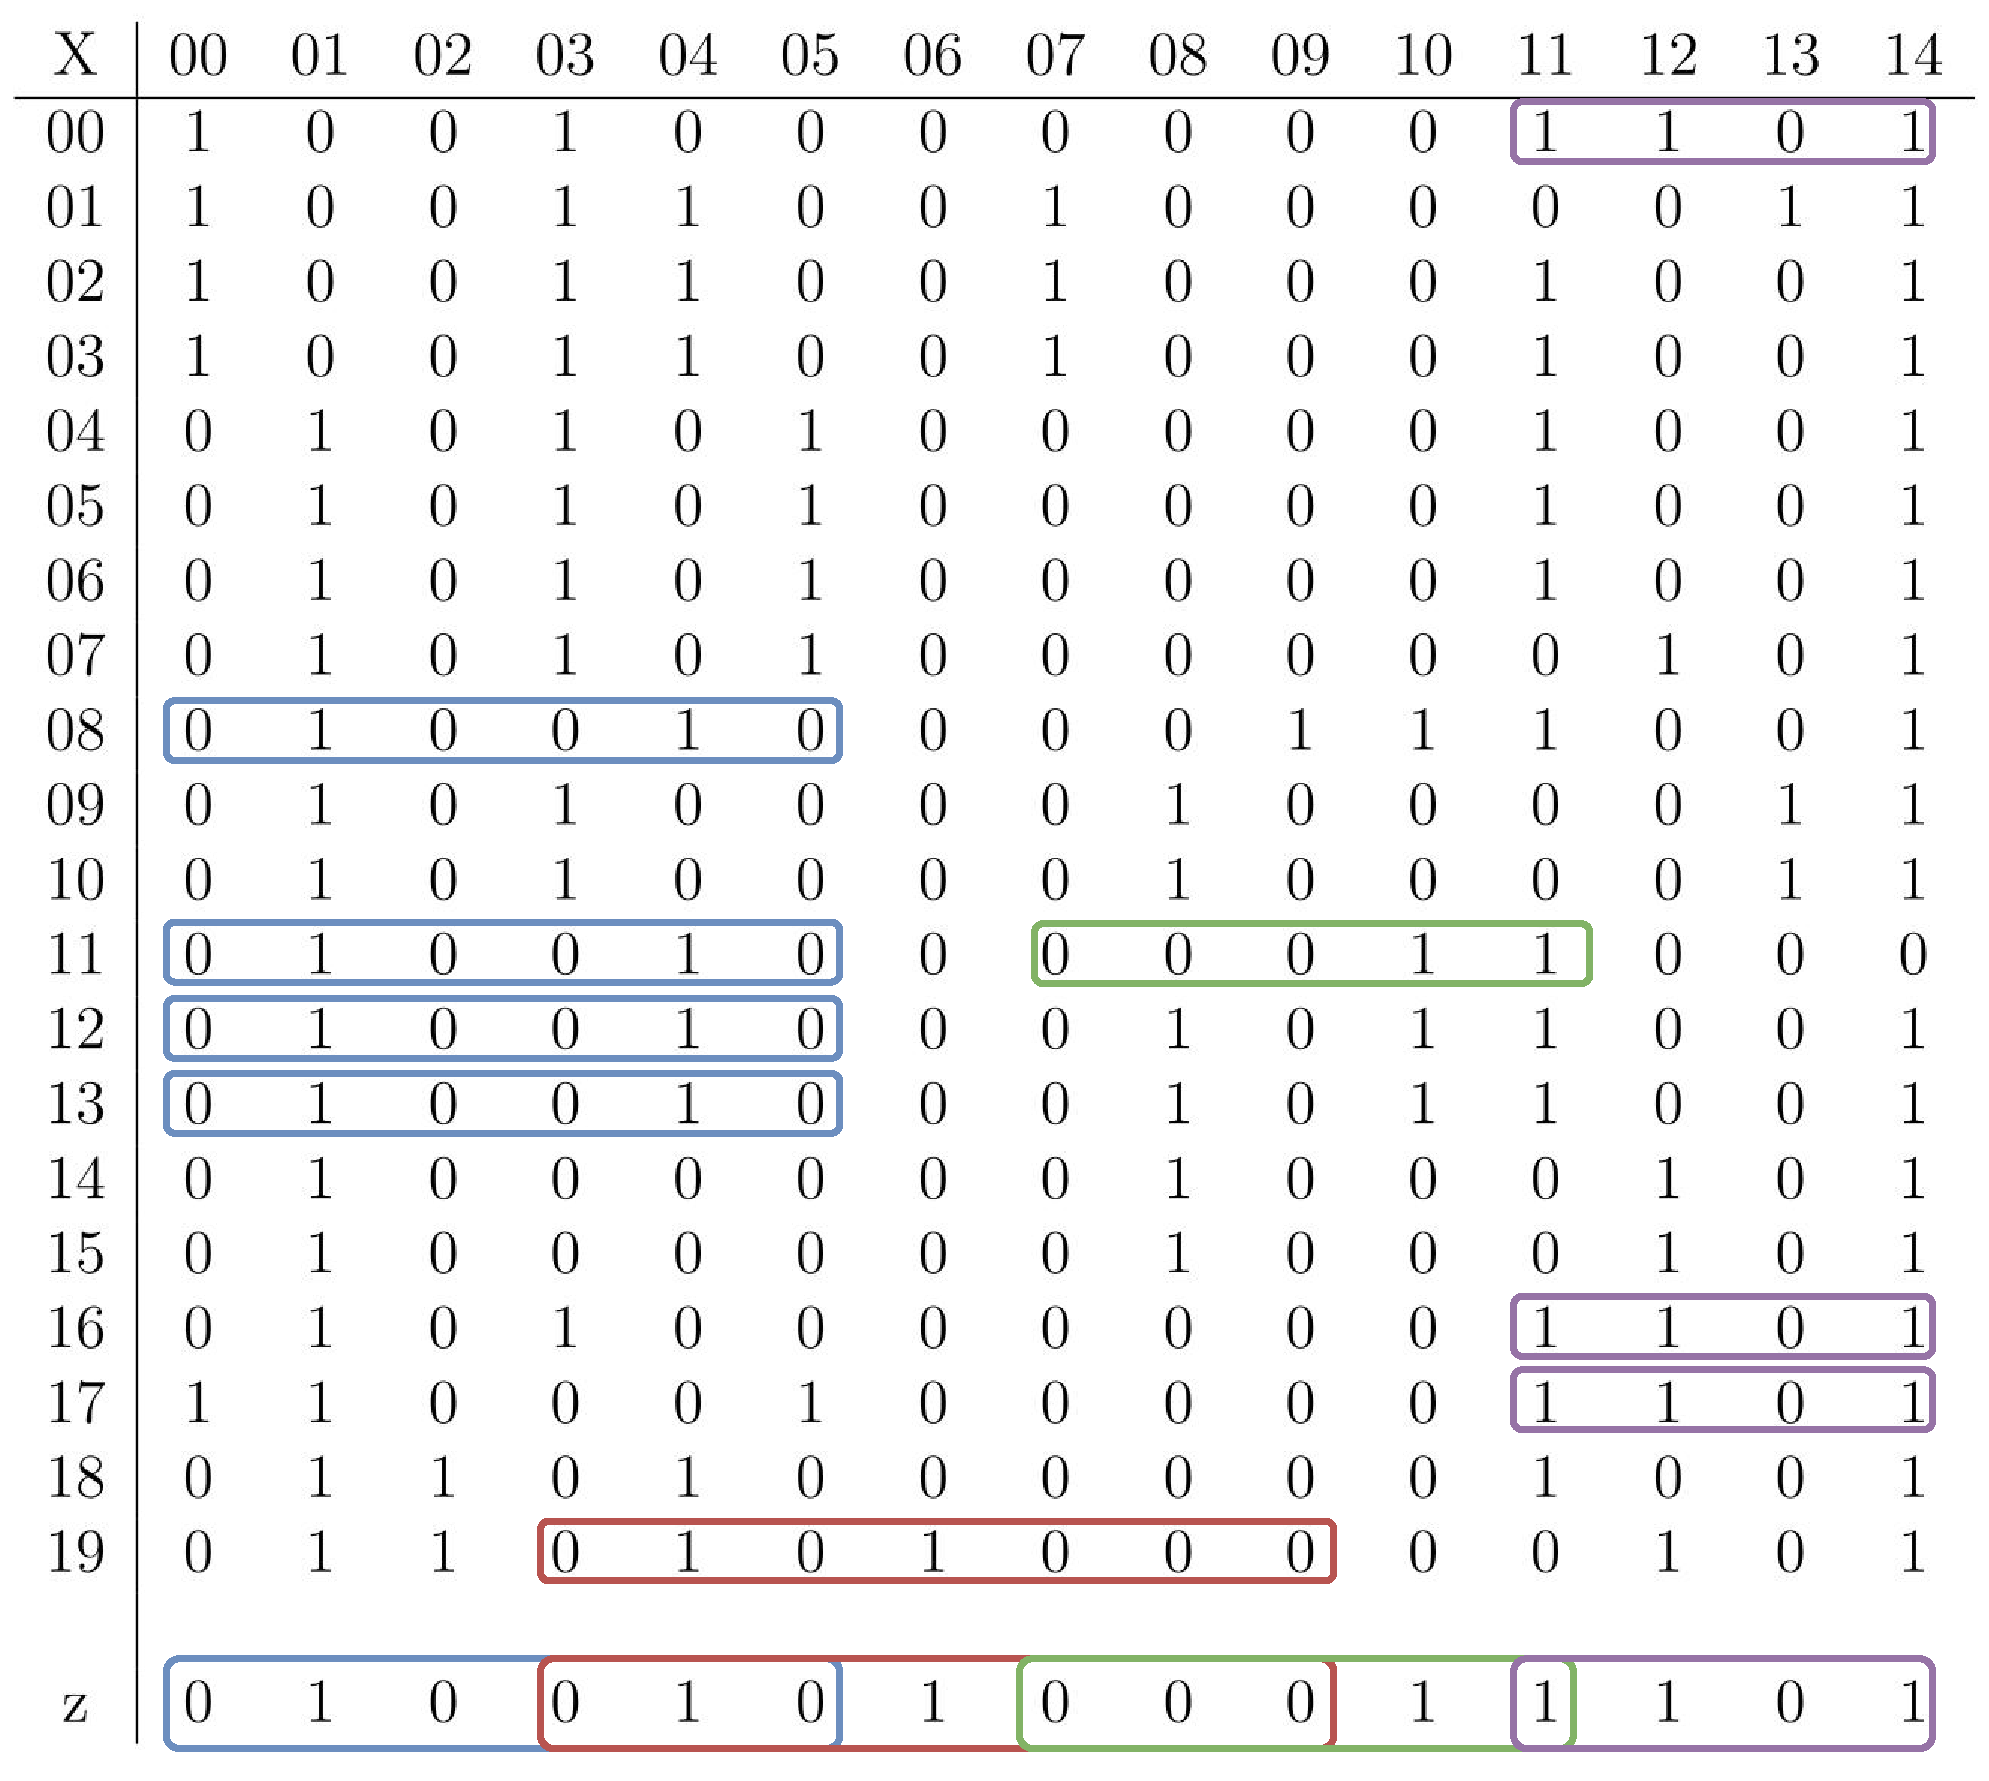
\includegraphics[scale = 0.27]{img/match.pdf}
  \end{figure}
\end{frame}
\section{The New Idea}
\begin{frame}{New Idea I}
  \only<1>{
    \begin{block}{Let's take a step back and get closer to Durbin's original
        idea.} 
      At the moment we save:
      \begin{itemize}
        \item the position of every head of a run
        \item a boolean to mark if the first run is composed by zeros or ones
        \item the $c$ value of the column
        \item a single value for $u$ and $v$ (that are as in Durbin)
        \item the whole \textit{divergence array}, actually the \textit{LCP
          array}, (\textbf{WIP}) 
      \end{itemize}
    \end{block}
  }
  \only<2>{
    \begin{figure}[H]
      \centering
      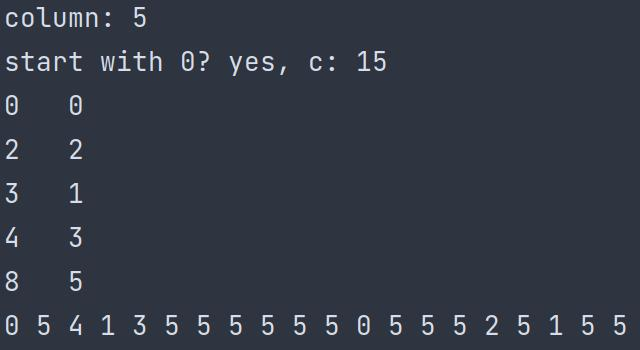
\includegraphics[scale = 0.4]{img/c5.jpg}
      \caption{Example, column 5: $00101111000000000000$}
    \end{figure}
  }
\end{frame}
\begin{frame}{New Idea II}
  \begin{block}{$uv$ values trick}
    Values $u$ and $v$ increase alternately in the biallelic case so we save
    every time the only value that increase at the head of a run.\\
    The, with a simple \textit{If/Else} selection based on the first element of
    the column and the index of the run and on being even or odd of the index we
    can extract both $u$ and $v$ values. Infact the two values are,
    alternatively, saved in the current index and in the previous one.
  \end{block}
  \begin{block}{$w(i,\sigma)$ function}
    We can use the same \textit{LF-mapping} as in Durbin but we have to consider
    sometimes an \textit{offset} between the position of the head of the run,
    that's $i$, which contains the ``virtual'' index, and the index itself.
    \[w(i,\sigma)=
      \begin{cases}
        u[i]+offset&\mbox{if } \sigma=0\\
        c+v[i]+offset&\mbox{if } \sigma=1\\
      \end{cases}
    \]
  \end{block}
\end{frame}
\begin{frame}{New Idea III}
  \begin{block}{External haplotype matches}
    Than we proceed as in Durbin, updating $f$ and $g$ using $w(i,\sigma)$.\\
    Every time we ``virtually'' use indexes over the whole column but actually
    run heads plus offsets are used. \\
    In case we update $e$ using $f$ and the \textit{divergence/LCP array}
    (\textbf{WIP}).\\
    In order to update $e$ we should in theory follow the line indicated in $i +
    1$ by $f$ in the original panel which we have not memorized. So, at most at
    a cost of $O(r)$ for every column, we proceed to reverse te use of $u$ and
    $v$ to move backwards between the columns virtually following a row of the
    original panel.\\
    Than we use the \textit{divergence/LCP array} (\textbf{WIP}) to update
    $f$ 
    and $g$ depending on the case.\\
    After detect a match, we can know the cardinality of the lines that match
    but not what they are, 
  \end{block}
\end{frame}
\begin{frame}{New Idea IV}
  \begin{block}{WIP}
    At the moment \textit{divergence array} is saved as an
    \texttt{sdsl::int\_vector<>} on which it's used
    \texttt{sdsl::util::bit\_compress()} in order to save space.\\
    The original idea of thresholds seems to me absolutely not applicable but
    maybe we can think of storing only a subset of the \textit{divergence/LCP
      array} and I'm thinking how to do it.   
  \end{block}
\end{frame}
% \begin{frame}{Two Pass on RLPBWT}
%   \begin{block}{}
%     In order to not save the \textit{divergence/LCP array} we could make two
%     \textit{RLPBWT}, one for the normal order and one for the reverse order.
%   \end{block}
%   \begin{block}{}
%     Instead of use the \textit{divergence/LCP array} to retrieve matches
%     that are overlapped in the panel we look for non overlapped matches only.\\
%     To do this when we find a match we continue the search updating $f$ and $g$
%     based only on $c$ and $h$, the total number of haplotypes in the panel:
%     \[(f,g)=
%       \begin{cases}
%         (0, c) & \mbox{if } \sigma=0\\
%         (c, h) & \mbox{if } \sigma=1
%       \end{cases}
%     \]
%   \end{block}
%   \begin{block}{}
%     We query in this way the first one with the haplotype and the second one
%     with the reverse of the haplotype. Than we intersect the results.
%   \end{block}
% \end{frame}
% \begin{frame}{Two Pass on RLPBWT}
%   \only<1>{
%     \begin{figure}[H]
%       \centering
%       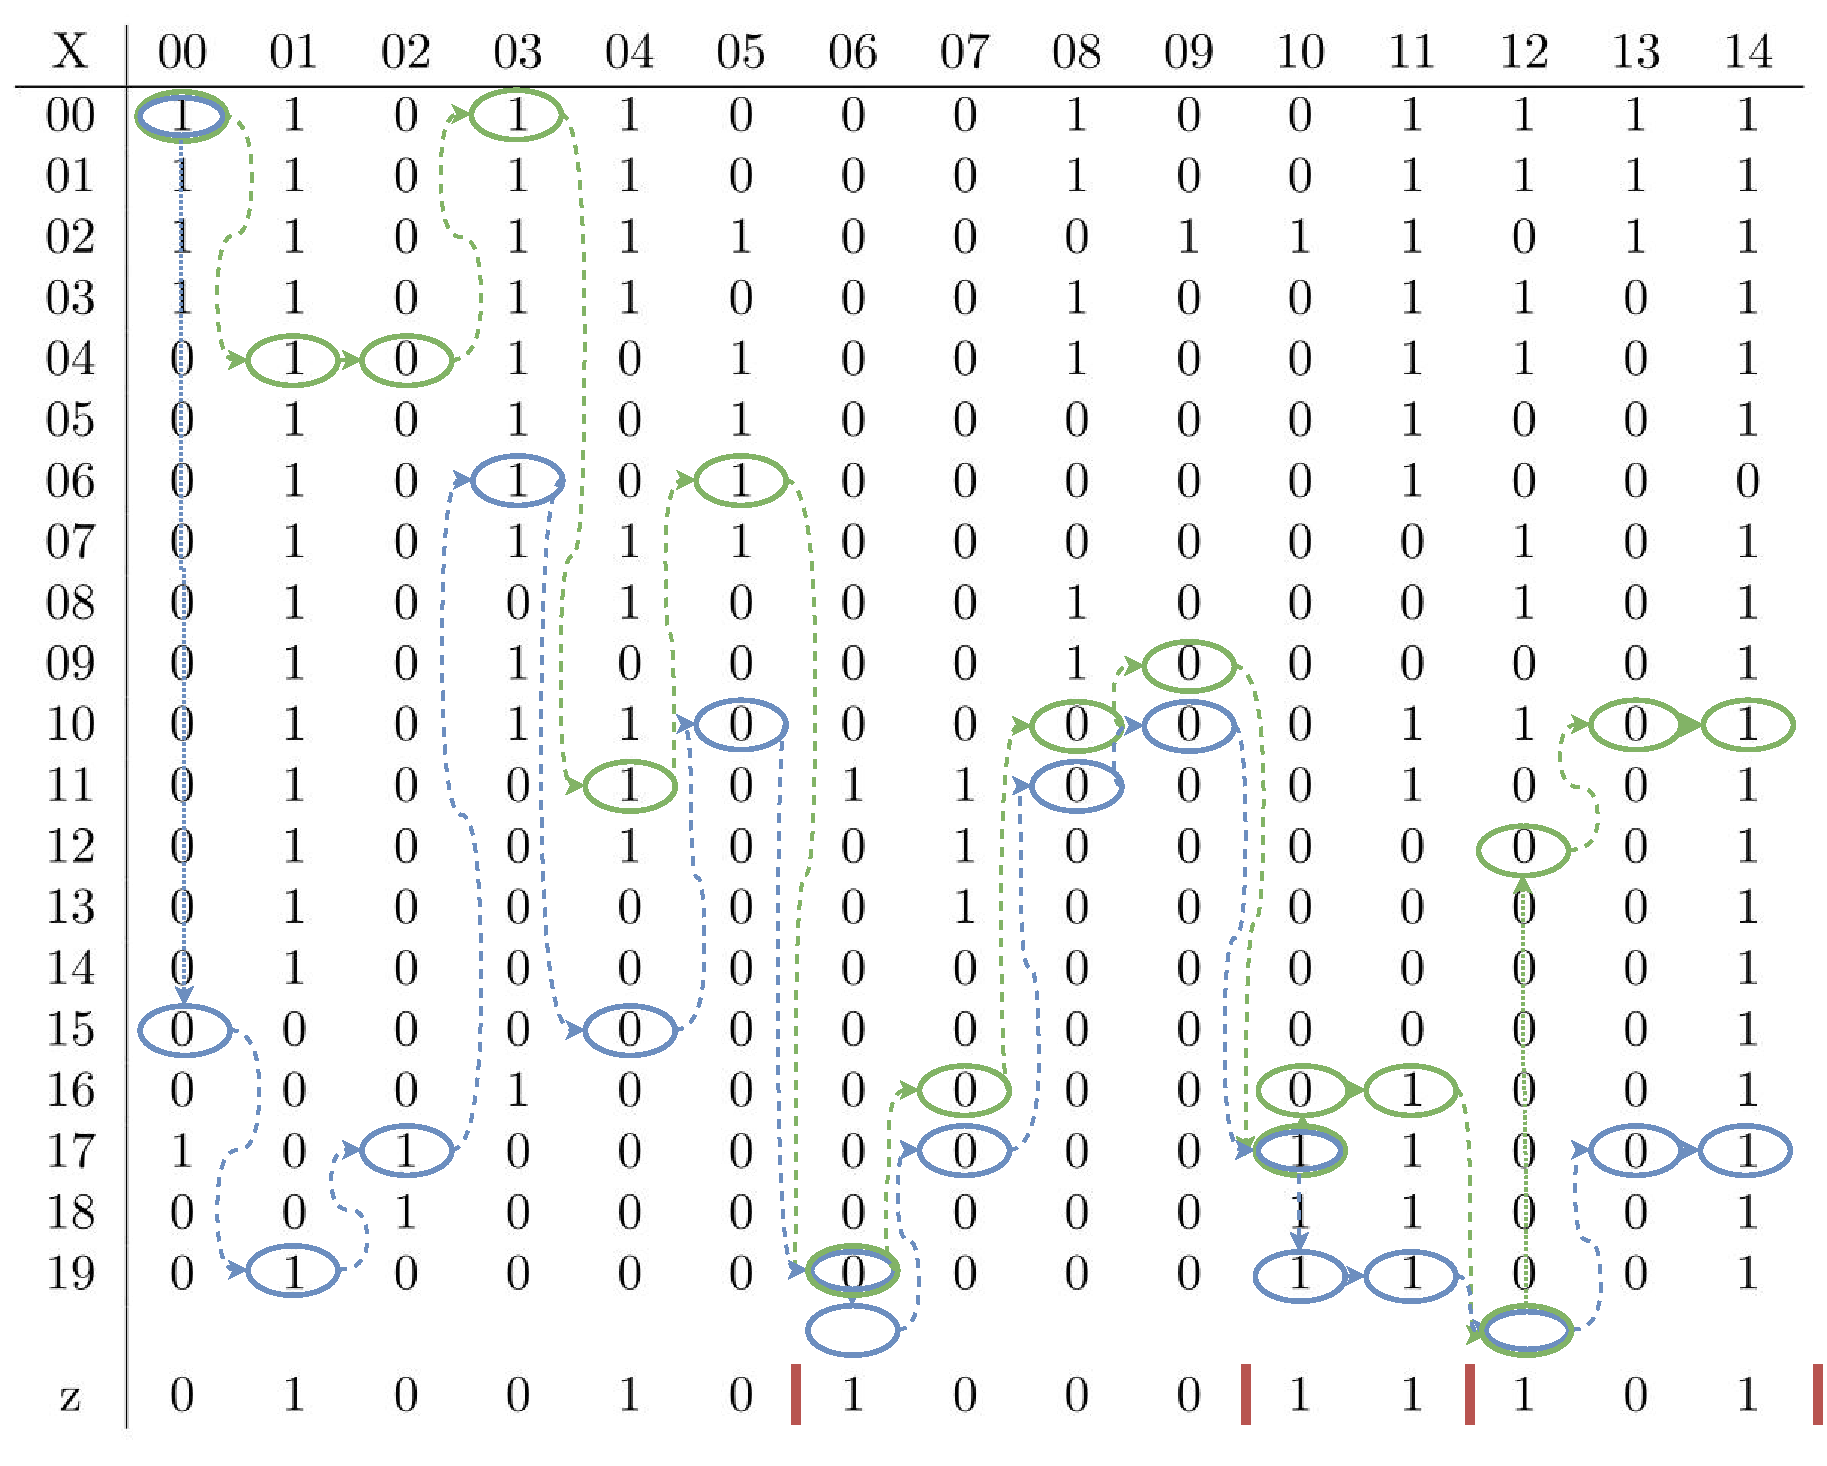
\includegraphics[scale = 0.3]{graph/bifronttravis.pdf}
%     \end{figure}
%   }
%   \only<2>{
%     \begin{figure}[H]
%       \centering
%       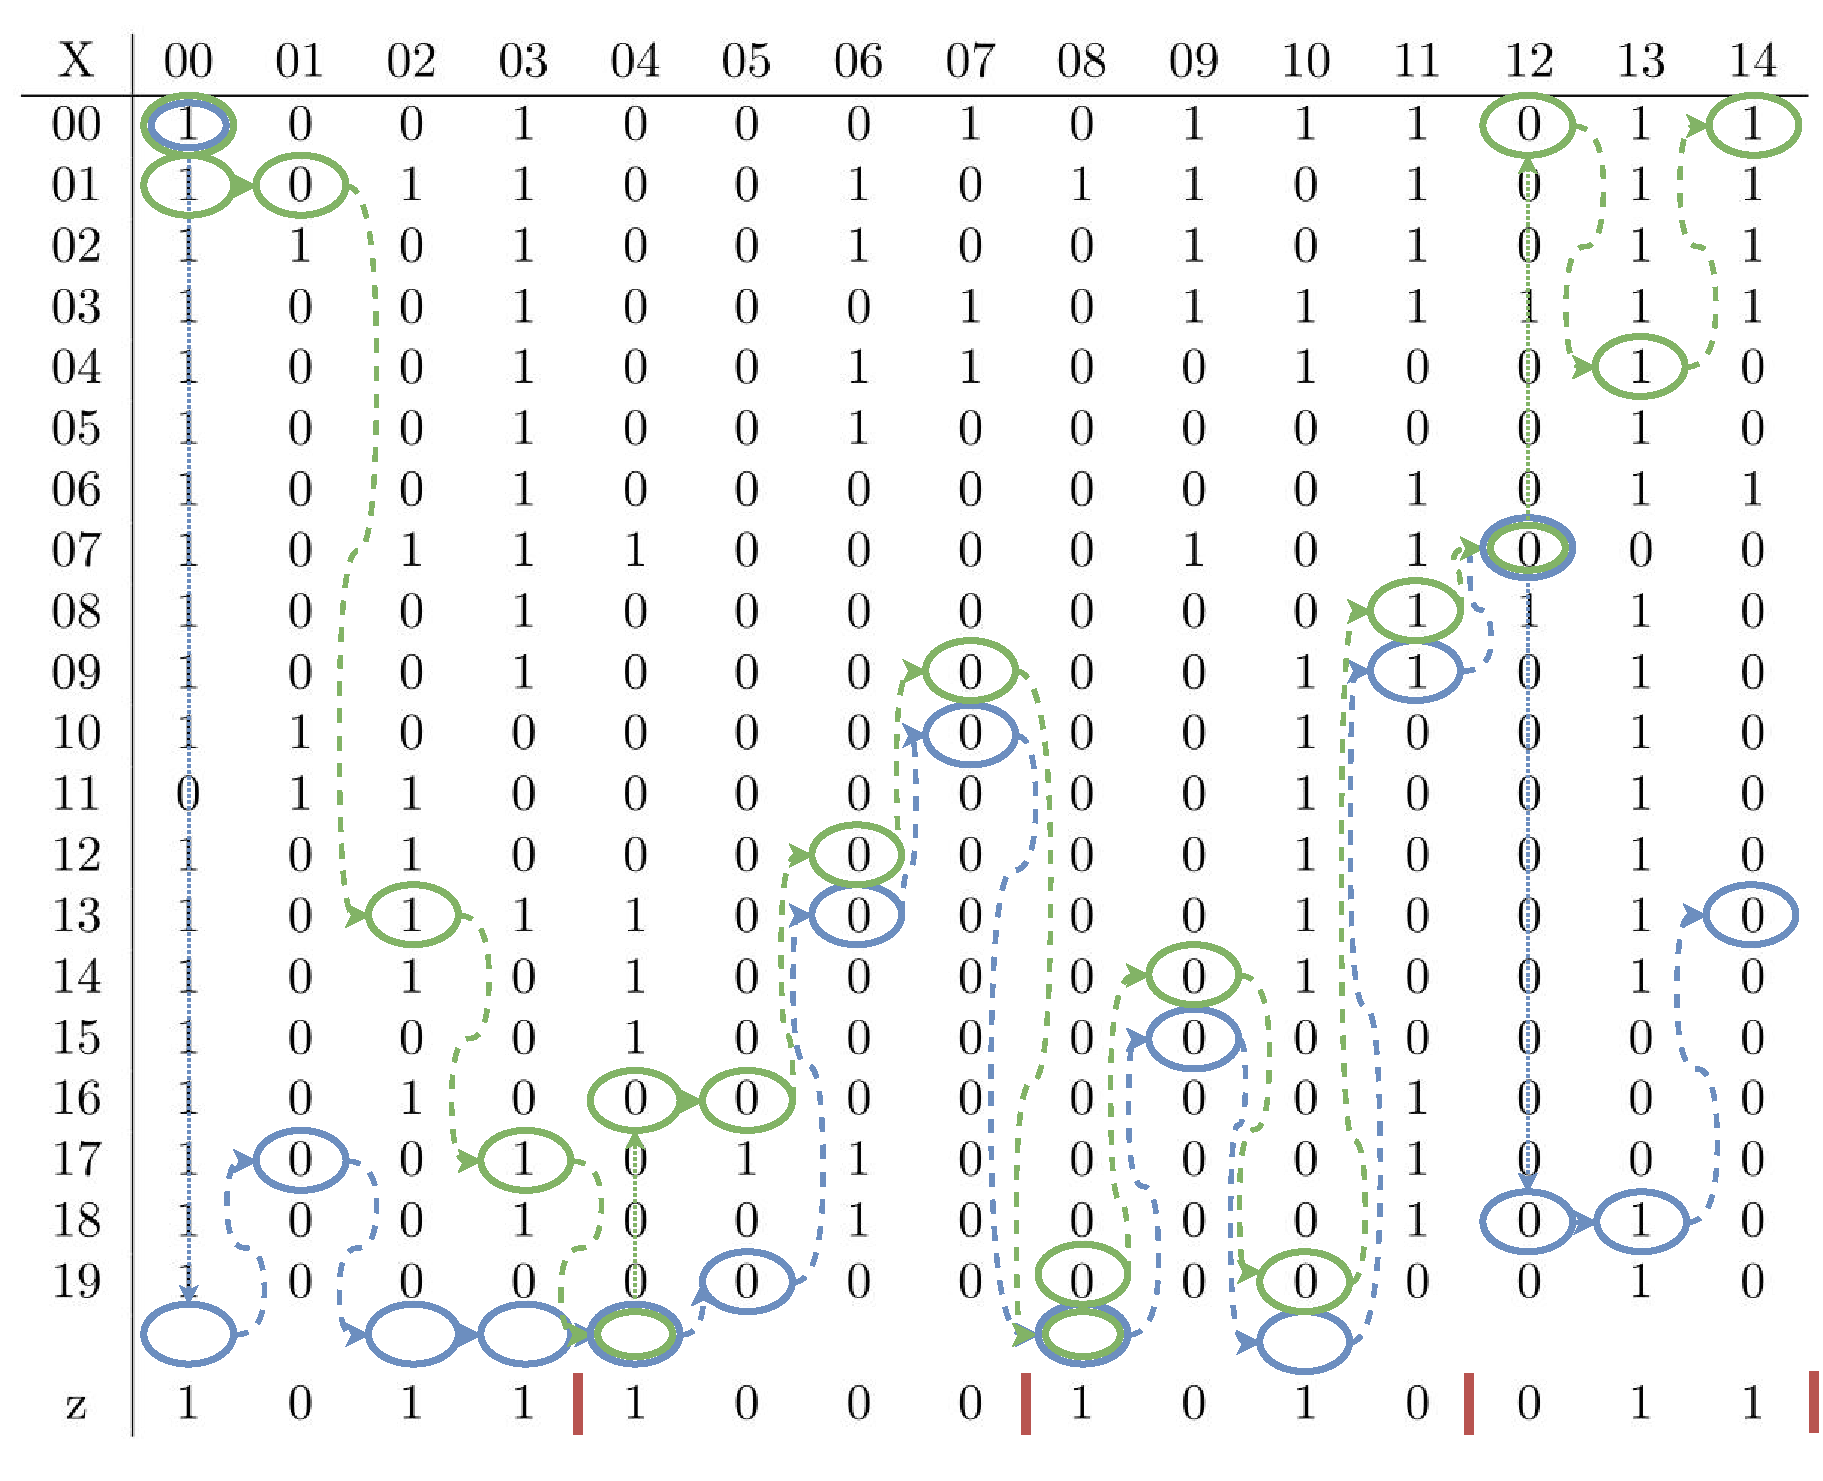
\includegraphics[scale = 0.3]{graph/bibacktravis.pdf}
%     \end{figure}
%   }
%   \only<3>{
%     \begin{figure}[H]
%       \centering
%       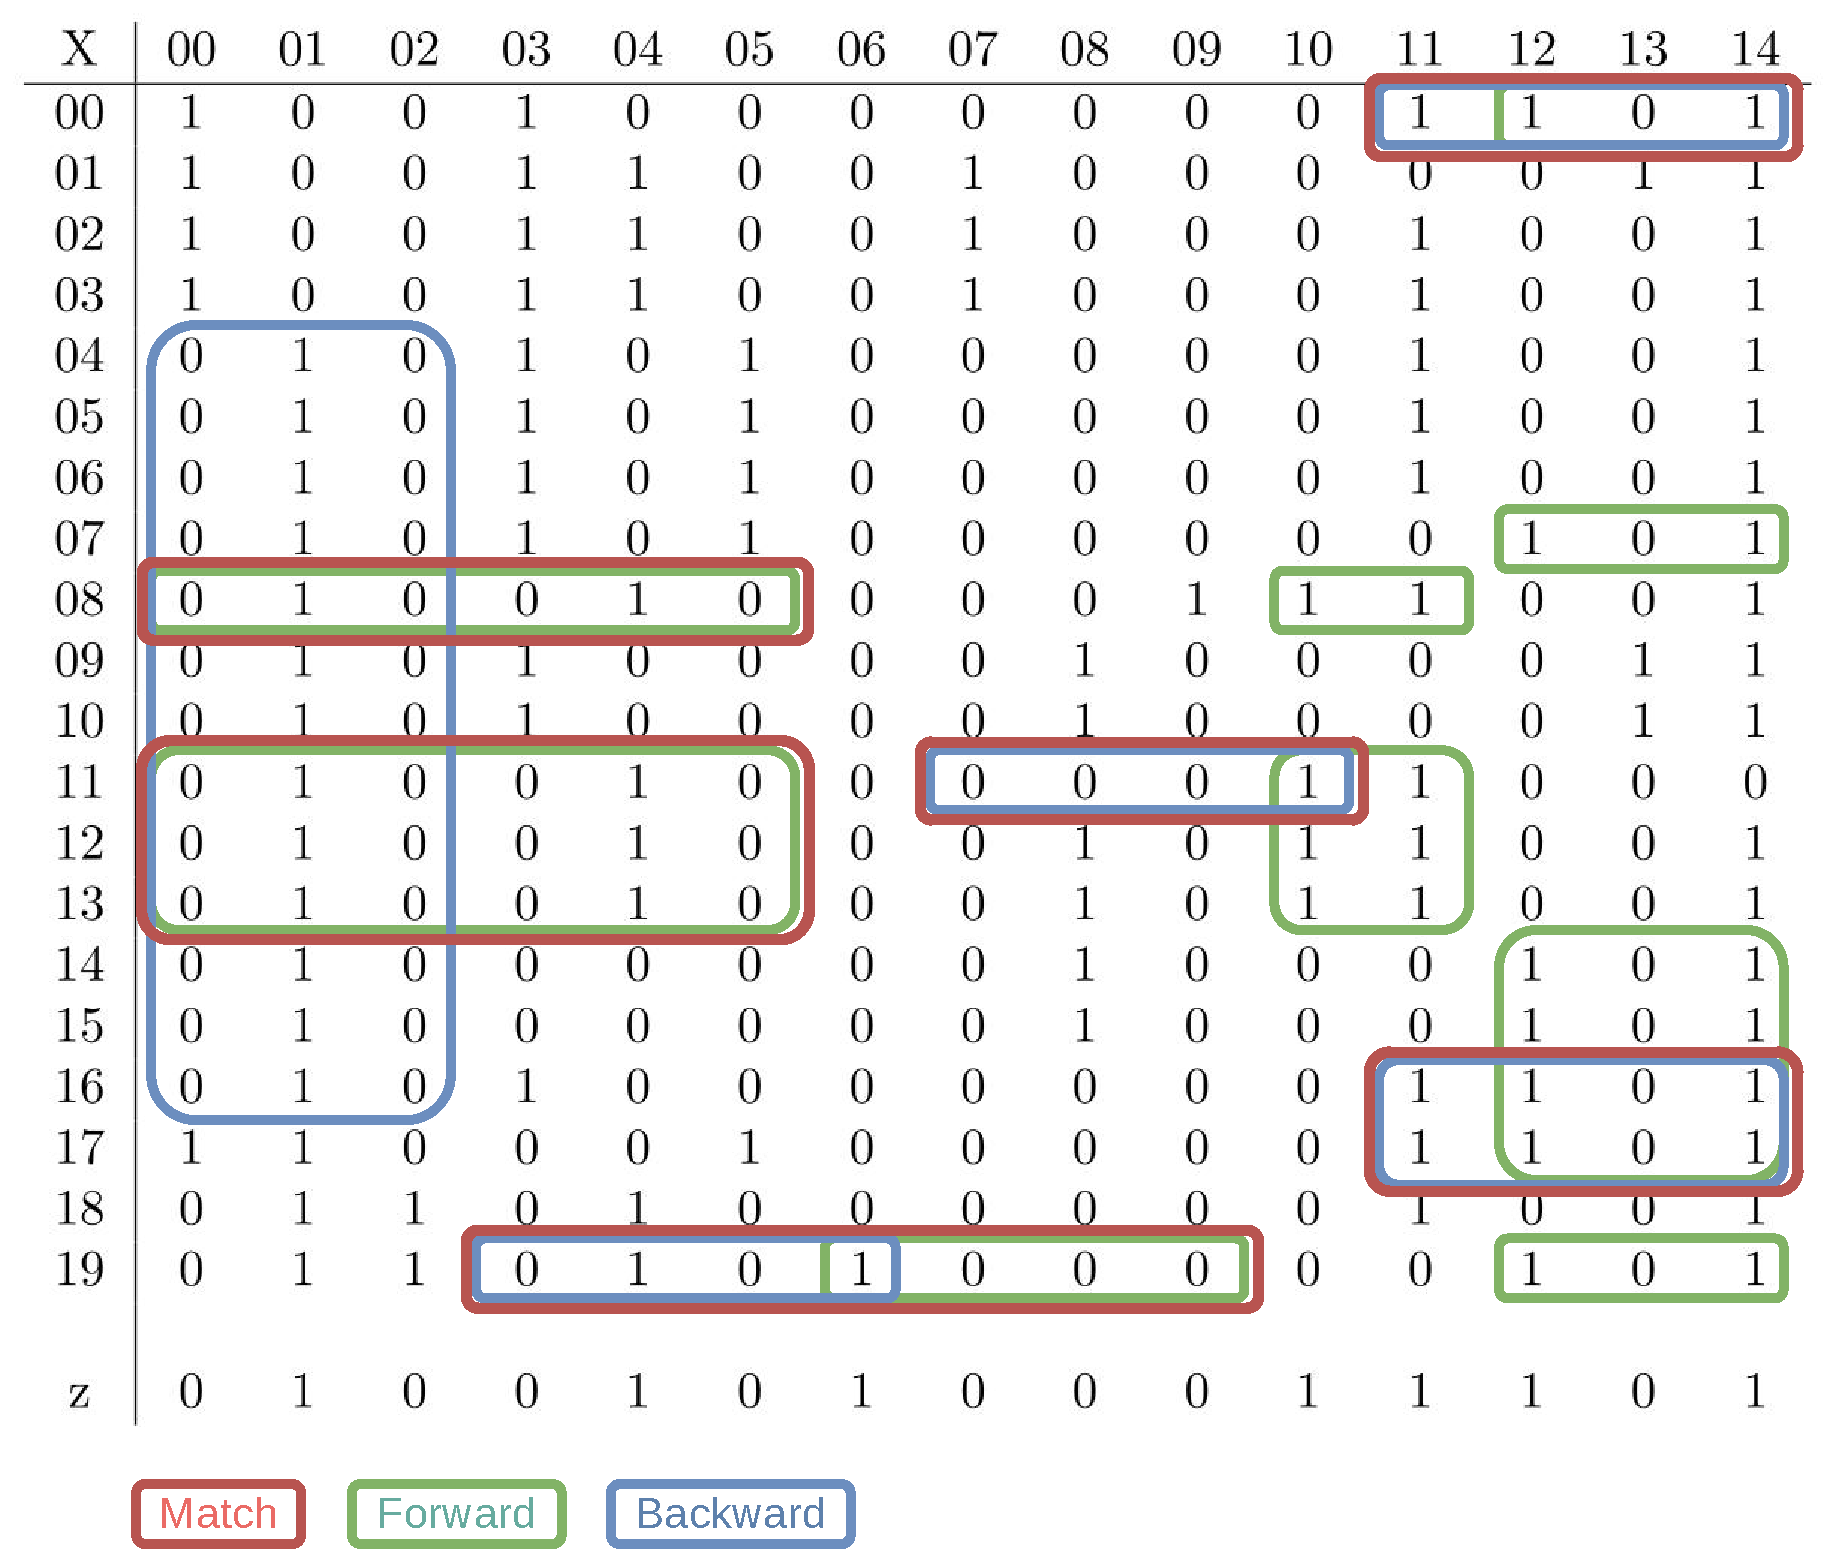
\includegraphics[scale = 0.3]{graph/bitravismatch.pdf}
%     \end{figure}
%   }
% \end{frame}
\begin{frame}{Testing}
  \begin{block}{Benchmark}
    At the moment I'm testing the implementation using the sample data (VCF
    files) at:\\
    \small{\color{nordred}
      \url{https://github.com/ZhiGroup/Syllable-PBWT/tree/master/sample_data}}\\
    (the panel is $900\times 500$ with $100$ queries). 
  \end{block}
  % \begin{alertblock}{Next Work}
  %   Trying to implement also non maximal matches with a query, as, for example,
  %   in Naseri's paper.
  % \end{alertblock}
\end{frame}
\section{BitVector Version}
\begin{frame}{The column data I}
  \begin{block}{}
    We save, for every column:
    \begin{itemize}
      \item a bit vector of the same length of the dense PBWT column, with 1 in
      every position before a head of a run
      \item 2 bit vector that can be queried to obtain $u$ and $v$ value. So we
      have a bitvector for zeros that contains 1 in position $i$ iff we have $i$
      zeros at point in the column when we change value anche similar for
      ones(\textbf{to be exaplained better})
      \item the $c$ value and a bool to indicate how a column start
    \end{itemize}
  \end{block}
\end{frame}
\begin{frame}{The column data II}
  \begin{block}{example}
    If we have a column:
    
    \[c=00001110001111110{\color{nordred}{0}}001111111\]
    We save:
    \[h=000100100100000100010000000(1)\]
    \[u=00010010001\mbox{ (to rappresent 4,3 and 4 zeros)}\]
    \[v=0010000010000001\mbox{ (to rappresent 3,6 and 7 ones)}\]
  \end{block}
\end{frame}
\begin{frame}{The column data III}
  \begin{block}{example}
    If we want to obtain, for example, the number of zeros before and index $i$,
    for example $i=18$:
    \begin{itemize}
      \item we \textit{rank} $h$ to obtain the run that contain $i$,
      $rank_h(18)= 4$ 
      \item we know that the column start with 0 so we are in a run of zeros and
      we have $\lfloor\frac{4}{2}\rfloor = 2$ run's of zeros before
      \item we know that the number of zeros in the previous complete runs is
      $select_u(2)+1 = 7$
      \item remain zeros in the run to compute are given by $i-(select_h(4)+1)$
    \end{itemize}
  \end{block}
\end{frame}
% \begin{frame}{Idea to change the use of whole lcp array}
%   \begin{block}{}
%     When we have an ending match, discovered in $k+1$, with $f$ and $g-1$ in $k$,
%     we could: 
%     \begin{itemize}
%       \item take maximum lcp between $f$ and first $0/1$ above $f$
%       \item take maximum lcp between $g$ and first $0/1$ below $g-1$
%       \item take maximum between these two values, we call it $x$
%       \item new interval is $[psv[x],\,\, nsv[x]-1]$ and we use this value to
%       obtain new $e$
%     \end{itemize}
%   \end{block}
%   \begin{alertblock}{}
%     We could obtain $psv$ and $nsv$ array using \textit{RMQ} of
%     \textit{sdsl-lite}. \\
%     In future we will use thresholds.
%   \end{alertblock}
% \end{frame}
\section{Matching Statistics}
\begin{frame}{Matching Statistics and RLPBWT}
  \begin{block}{Some definitions}
    \begin{itemize}
      \item for every run in a column of the PBTW with define the
      \textbf{threshold} as the index of the minimum \textit{lcp value} (and we
      save it as a sparse bitvector of the same length of a column with 1 in
      these positions)
      \item for every run in a column of the PBTW with define the
      \textbf{prefix array samples} as the prefix array value at the begin of the
      run and at the end
      \item we define matching statistics as a two components ($row, len$) vector $MS$ of the
      same length of the query such that $\forall k\in[0,|z|)$: 
      \begin{itemize}
        \item $panel_{row}[k-(len+)1..k]=z[k-(len+1)..k]$
        \item $z[k-(len+1)..k+1]$ doesn't match with any row in the panel 
      \end{itemize}
      \item we need random access to the panel. At this time we are using a
      bitvector for every column of the panbel but we can use a data structure,
      called \textit{SLP}, with a very low memory cost but with high access times 
    \end{itemize}
  \end{block}
\end{frame}
\begin{frame}{Example}
  \begin{block}{Regarding the example seen above}
    \begin{table}[H]
      \footnotesize{}
      \centering
      \begin{tabular}{c|ccccccccccccccc}
        $k$ & 00 & 01 & 02 & 03 & 04 &  {\color{nordred}05} & 06 & 07 & 08
        &  {\color{nordgreen}09} & 10 &  {\color{nordgreen}11} & 12 & 13
        &  {\color{nordgreen}14} \\
        \hline
        $z$ & 0 & 1 & 0 & 0 & 1 &  {\color{nordgreen}0} & 1 & 0 & 0
        &  {\color{nordgreen}0} & 1 &  {\color{nordgreen}1} & 1 & 0
        &  {\color{nordgreen}1} \\
        $row$ & 19 & 19 & 17 & 17 & 13 &  {\color{nordgreen}13} & 19 & 19 & 19
        &  {\color{nordgreen}19} & 11 &  {\color{nordgreen}11} & 17 & 17
        &  {\color{nordgreen}17} \\
        $len$ & 1 & 2 & 3 & 4 & 5 & {\color{nordgreen}6} & 4 & 5 & 6
        & {\color{nordgreen}7} & 4 & {\color{nordgreen}5} & 2 & 3
        & {\color{nordgreen}4}\\
      \end{tabular}
    \end{table}
\end{block}
\end{frame}
          %           \begin{frame}[allowframebreaks]{References} 
          %           \nocite{*}
%   \bibliographystyle{unsrt}
%   \bibliography{ref}
% \end{frame}

\end{document}


